    \chapter{User Interface Design}\label{chap:ui}
    
    DREAM is a web-based application. It could be utilized on a variety of devices, independent of form factor. The application, however, is expected to be largely utilized on desktop computers. As a result, the given mockups depict representations of the application's desktop version.
    
    This chapter provides pictures of all the  mockups, that will be later used for the requirements traceability (see chapter \ref{ch:requirements_traceability}).
    
    \subsubsection{Unregistered user}
    
    The user can navigate to the sign-up screen using \textit{Create account} option, available in the horizontal navigation bar on the top of the page. After correctly filling the form, the user is redirected to the login page and receives a notification informing him about the success of the account creation process.
    \begin{figure}[H]
        \centering
        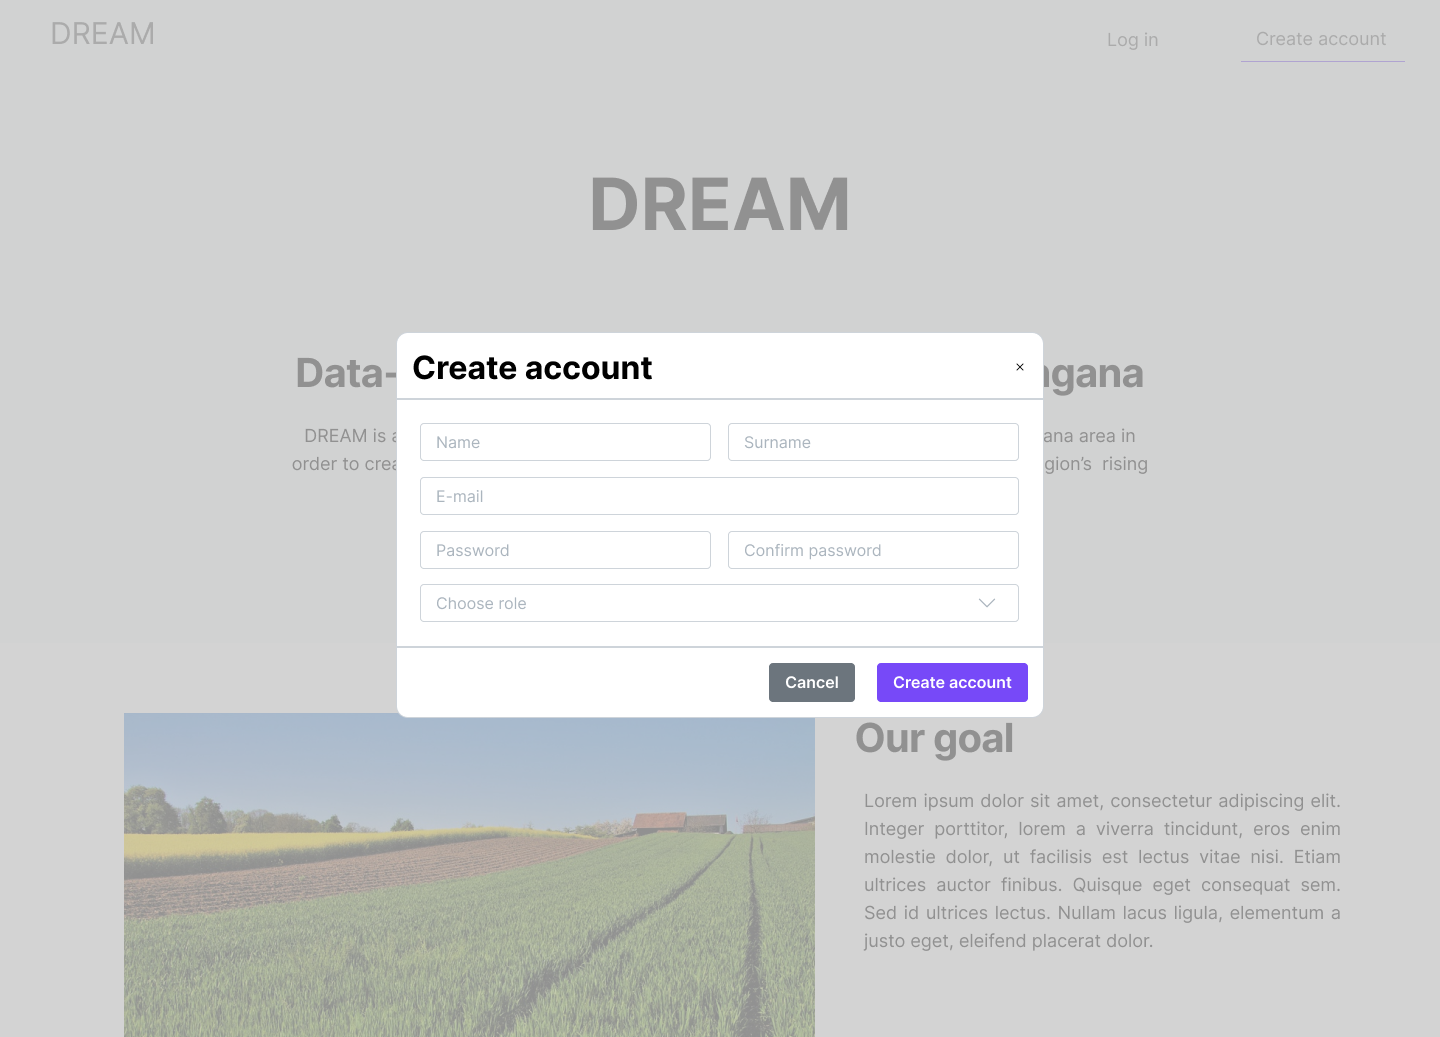
\includegraphics[width=0.75\textwidth]{mockups/Unreg. user_Create account.png}
        \caption{\textbf{M1.} User registration.}
        \label{fig:user-create-account}
    \end{figure}
    
    When the user chooses \textit{Farmer} role, additional fields appear, namely Sensor system's ID, Water irrigation system's ID, Address line 1, Address line 2, Postal code, City, and Mandal.
    \begin{figure}[H]
        \centering
        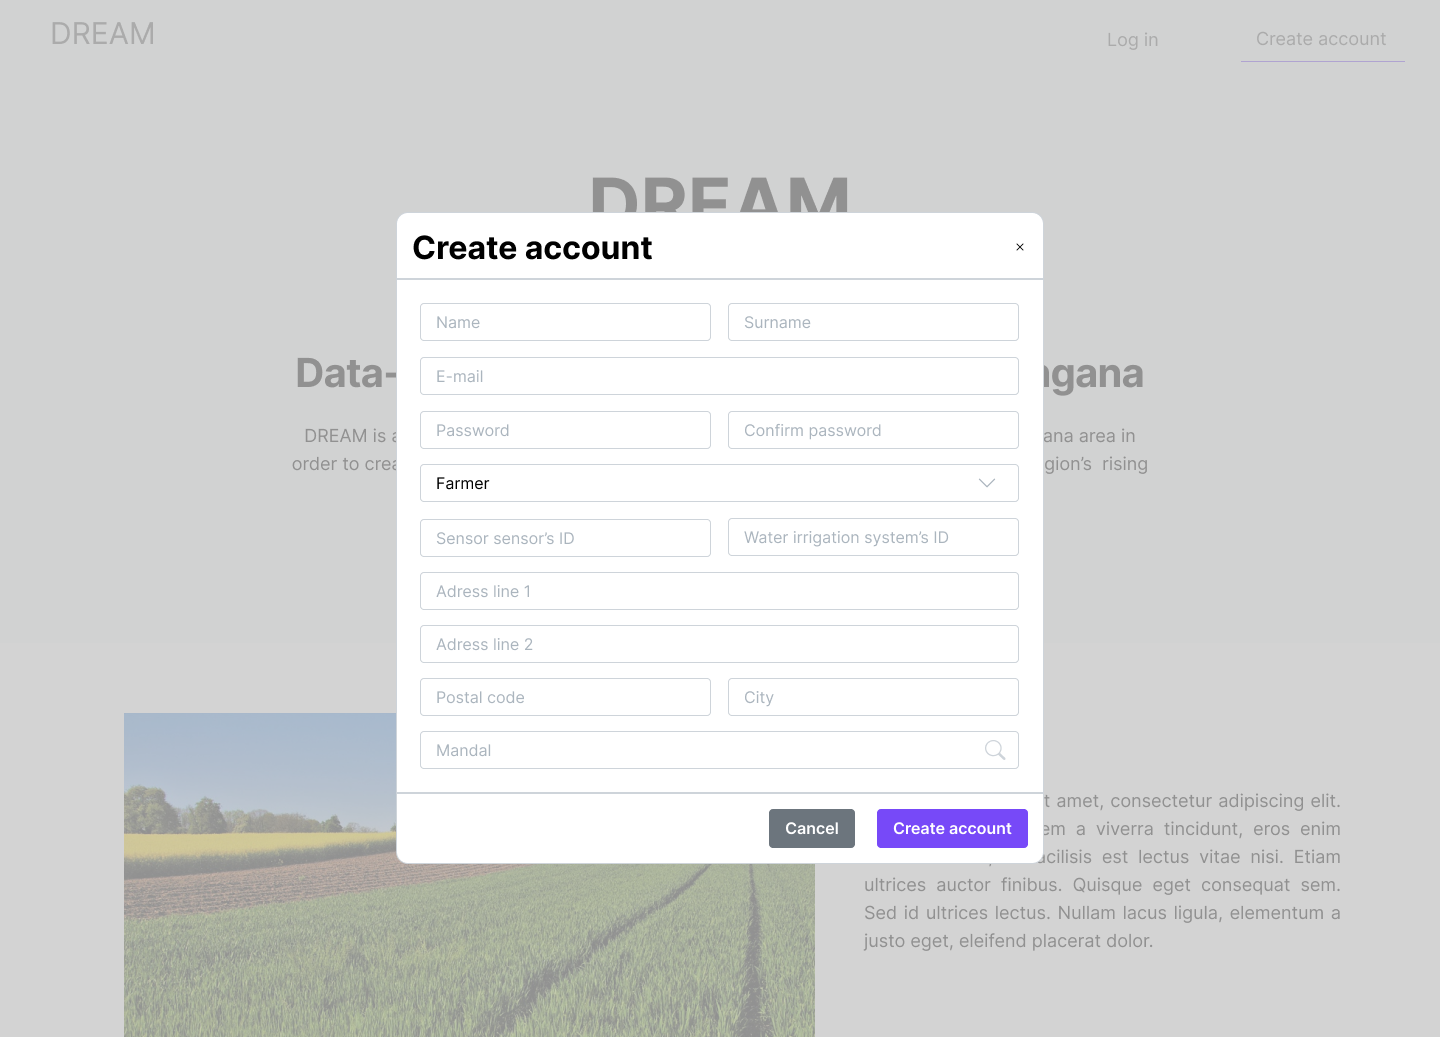
\includegraphics[width=0.75\textwidth]{mockups/Unreg. user_Create account_Farmer.png}
        \caption{\textbf{M2.} Farmer registration.}
        \label{fig:farmer-create-account}
    \end{figure}
    
    When the user chooses \textit{Agronomist} role, additional fields appear, allowing him to choose the area of responsibility.
    \begin{figure}[H]
        \centering
        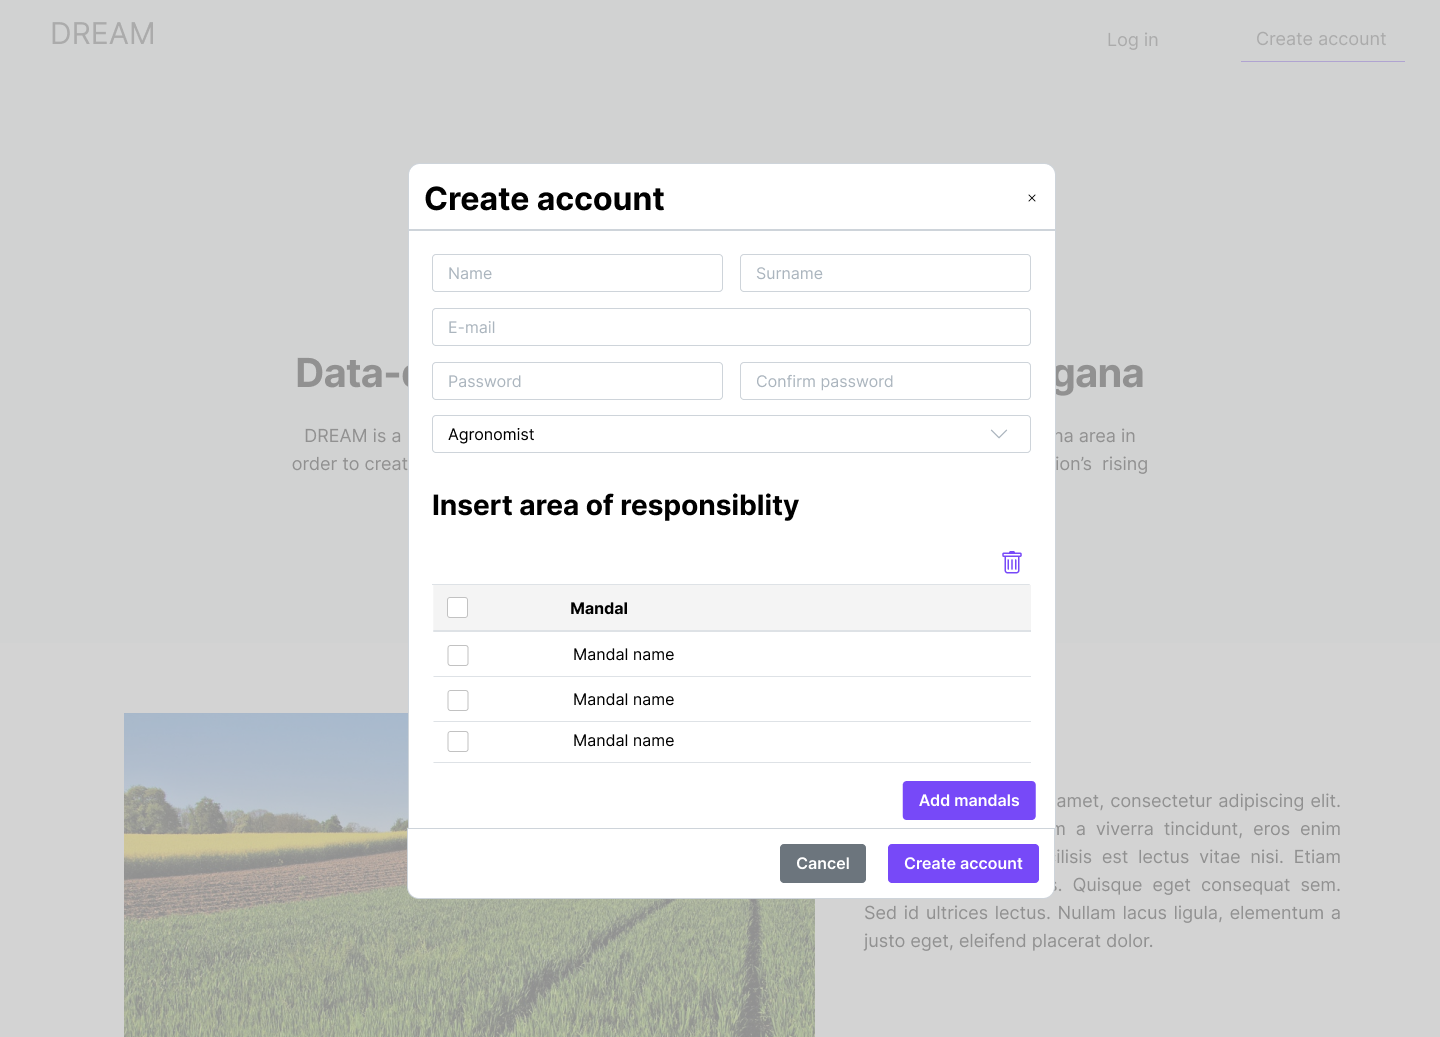
\includegraphics[width=0.75\textwidth]{mockups/Unreg. user_Create account_Agronomist.png}
        \caption{\textbf{M3.} Agronomist registration.}
        \label{fig:agronomist-create-account}
    \end{figure}
    
    The user can navigate to the log in screen using \textit{Log in} option, available in the horizontal navigation bar on the top of the page. It contains fields for providing e-mail and password. The user can also choose an option to remind a password, via a button in the lower part of the modal dialog.
    \begin{figure}[H]
        \centering
        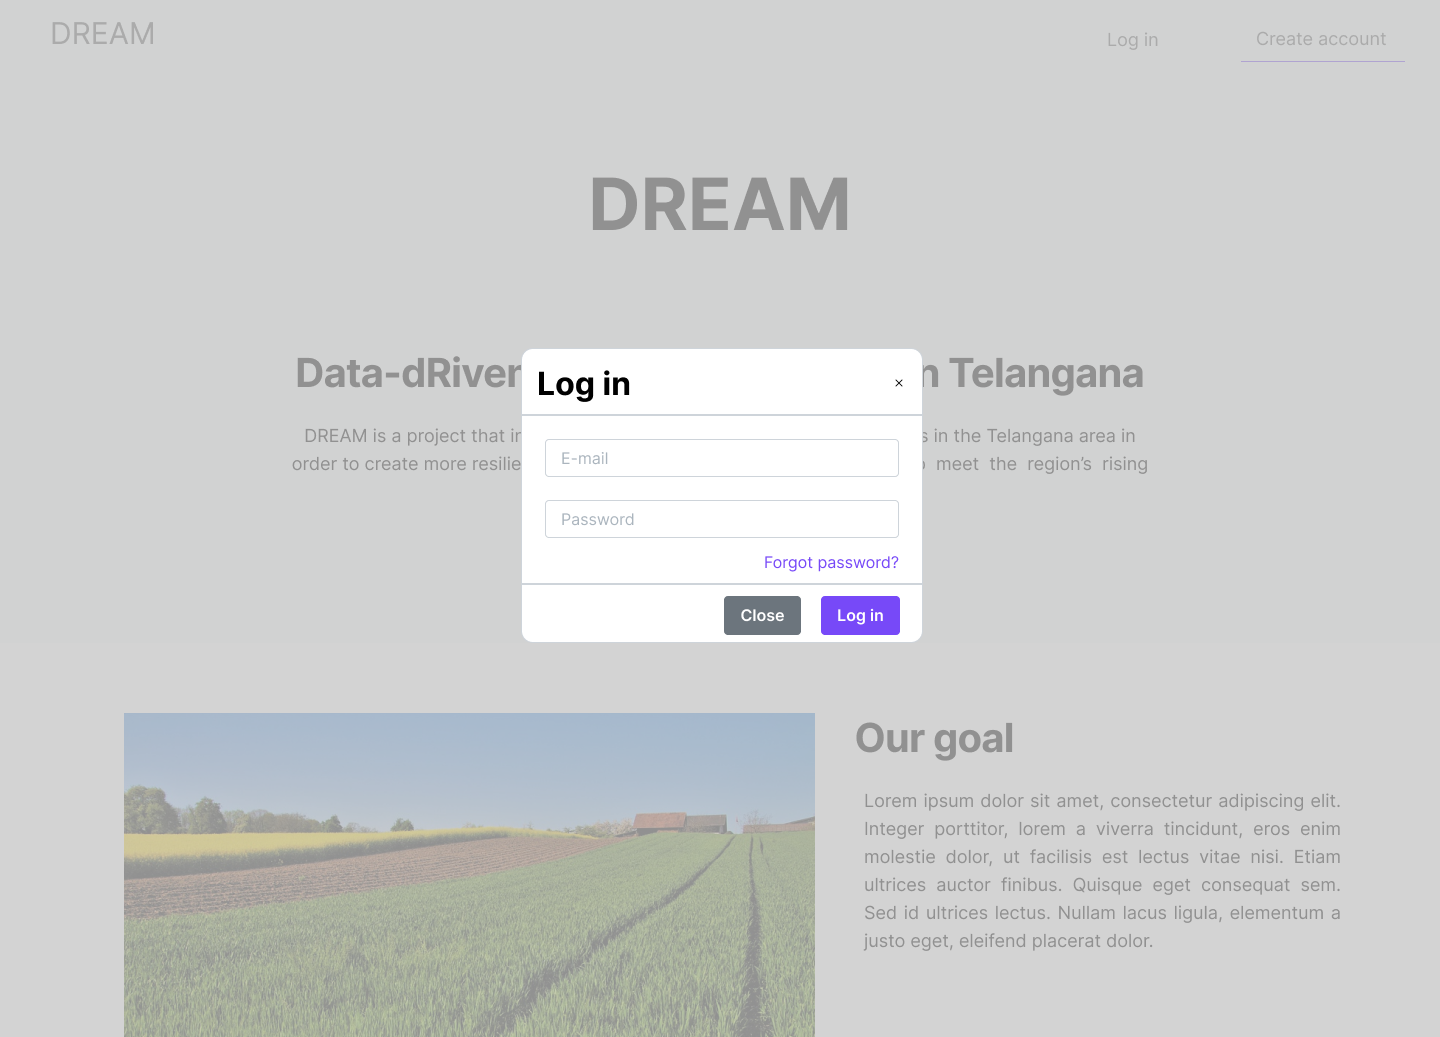
\includegraphics[width=0.75\textwidth]{mockups/Unreg. user_Log in.png}
        \caption{\textbf{M4.} Log in view.}
        \label{fig:user-log-in}
    \end{figure}
    
    The user can reset his password using the \textit{Remind password} view. He has to provide a valid e-mail address, to which the message will be sent.
    \begin{figure}[H]
        \centering
        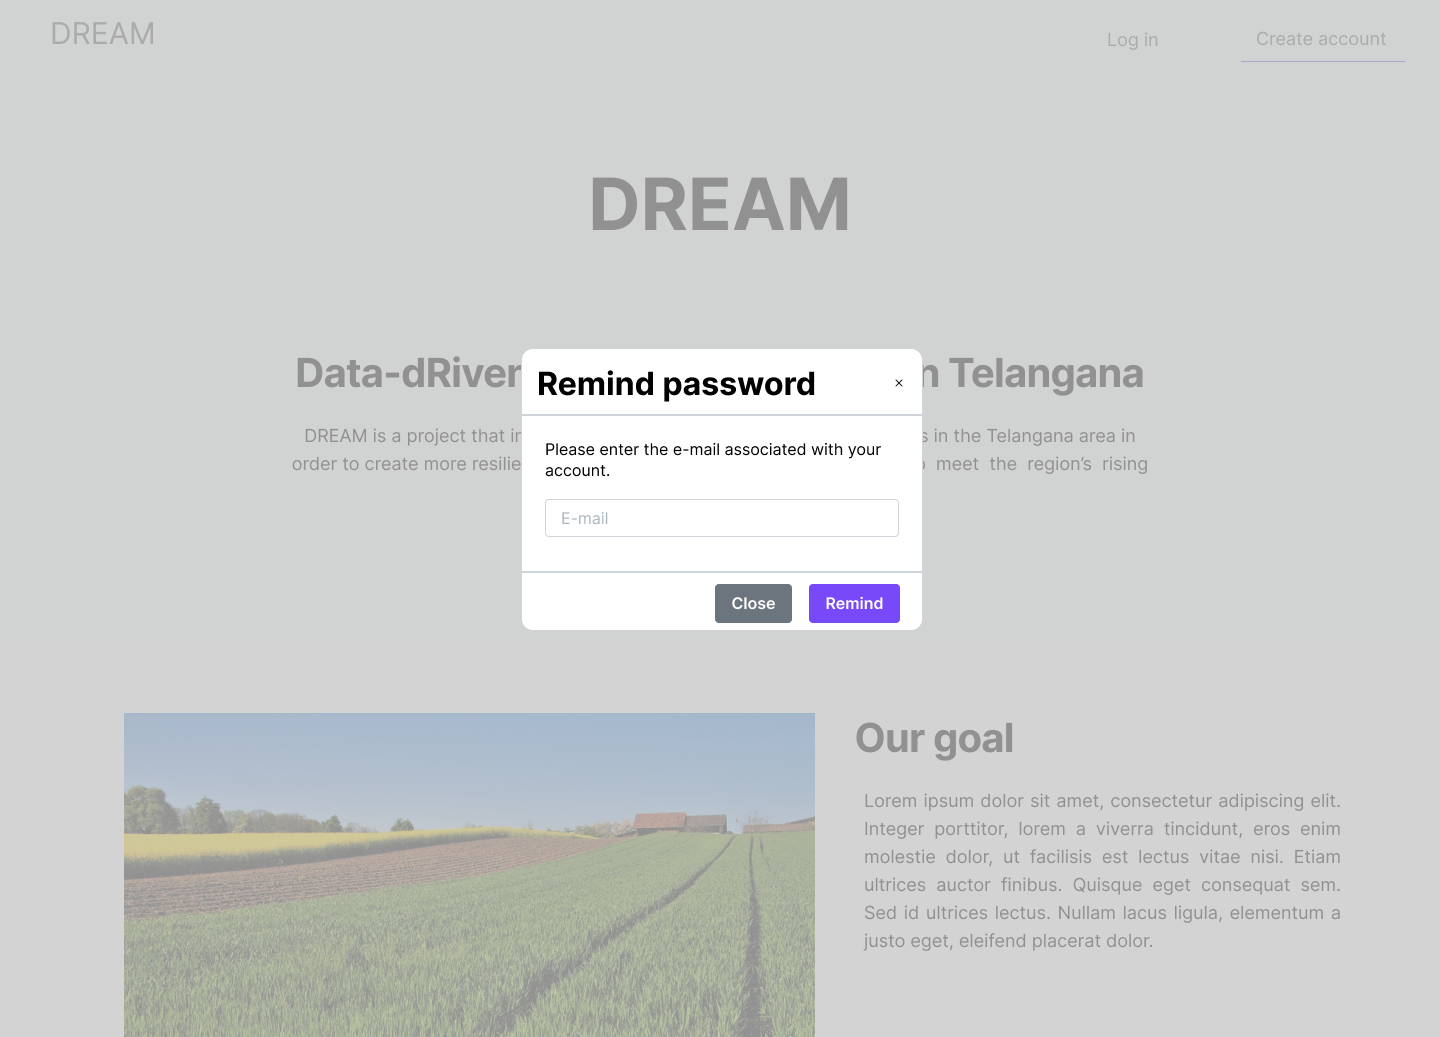
\includegraphics[width=0.75\textwidth]{mockups/Unreg. user_Remind password.png}
        \caption{\textbf{M5.} Remind password.}
        \label{fig:user-remind-password}
    \end{figure}
    
    
    \subsubsection{Farmer}
    
    Regardless of current view, a farmer can navigate to his summary, by clicking on the button containing his name and surname in the top navigation bar. The summary contains all the information about his account and farm. Following information are provided: account data, note history, production data, farm visits, weather, soil humidity, water usage, and help requests. User can see detailed view about farm visits and help requests, by clicking on the eye button in  a given table row. Farmer can also delete his account, using the \textit{Delete account} button in the bottom of the page and after confirming his choice in a modal pop-up. 
    \begin{figure}[H]
        \centering
        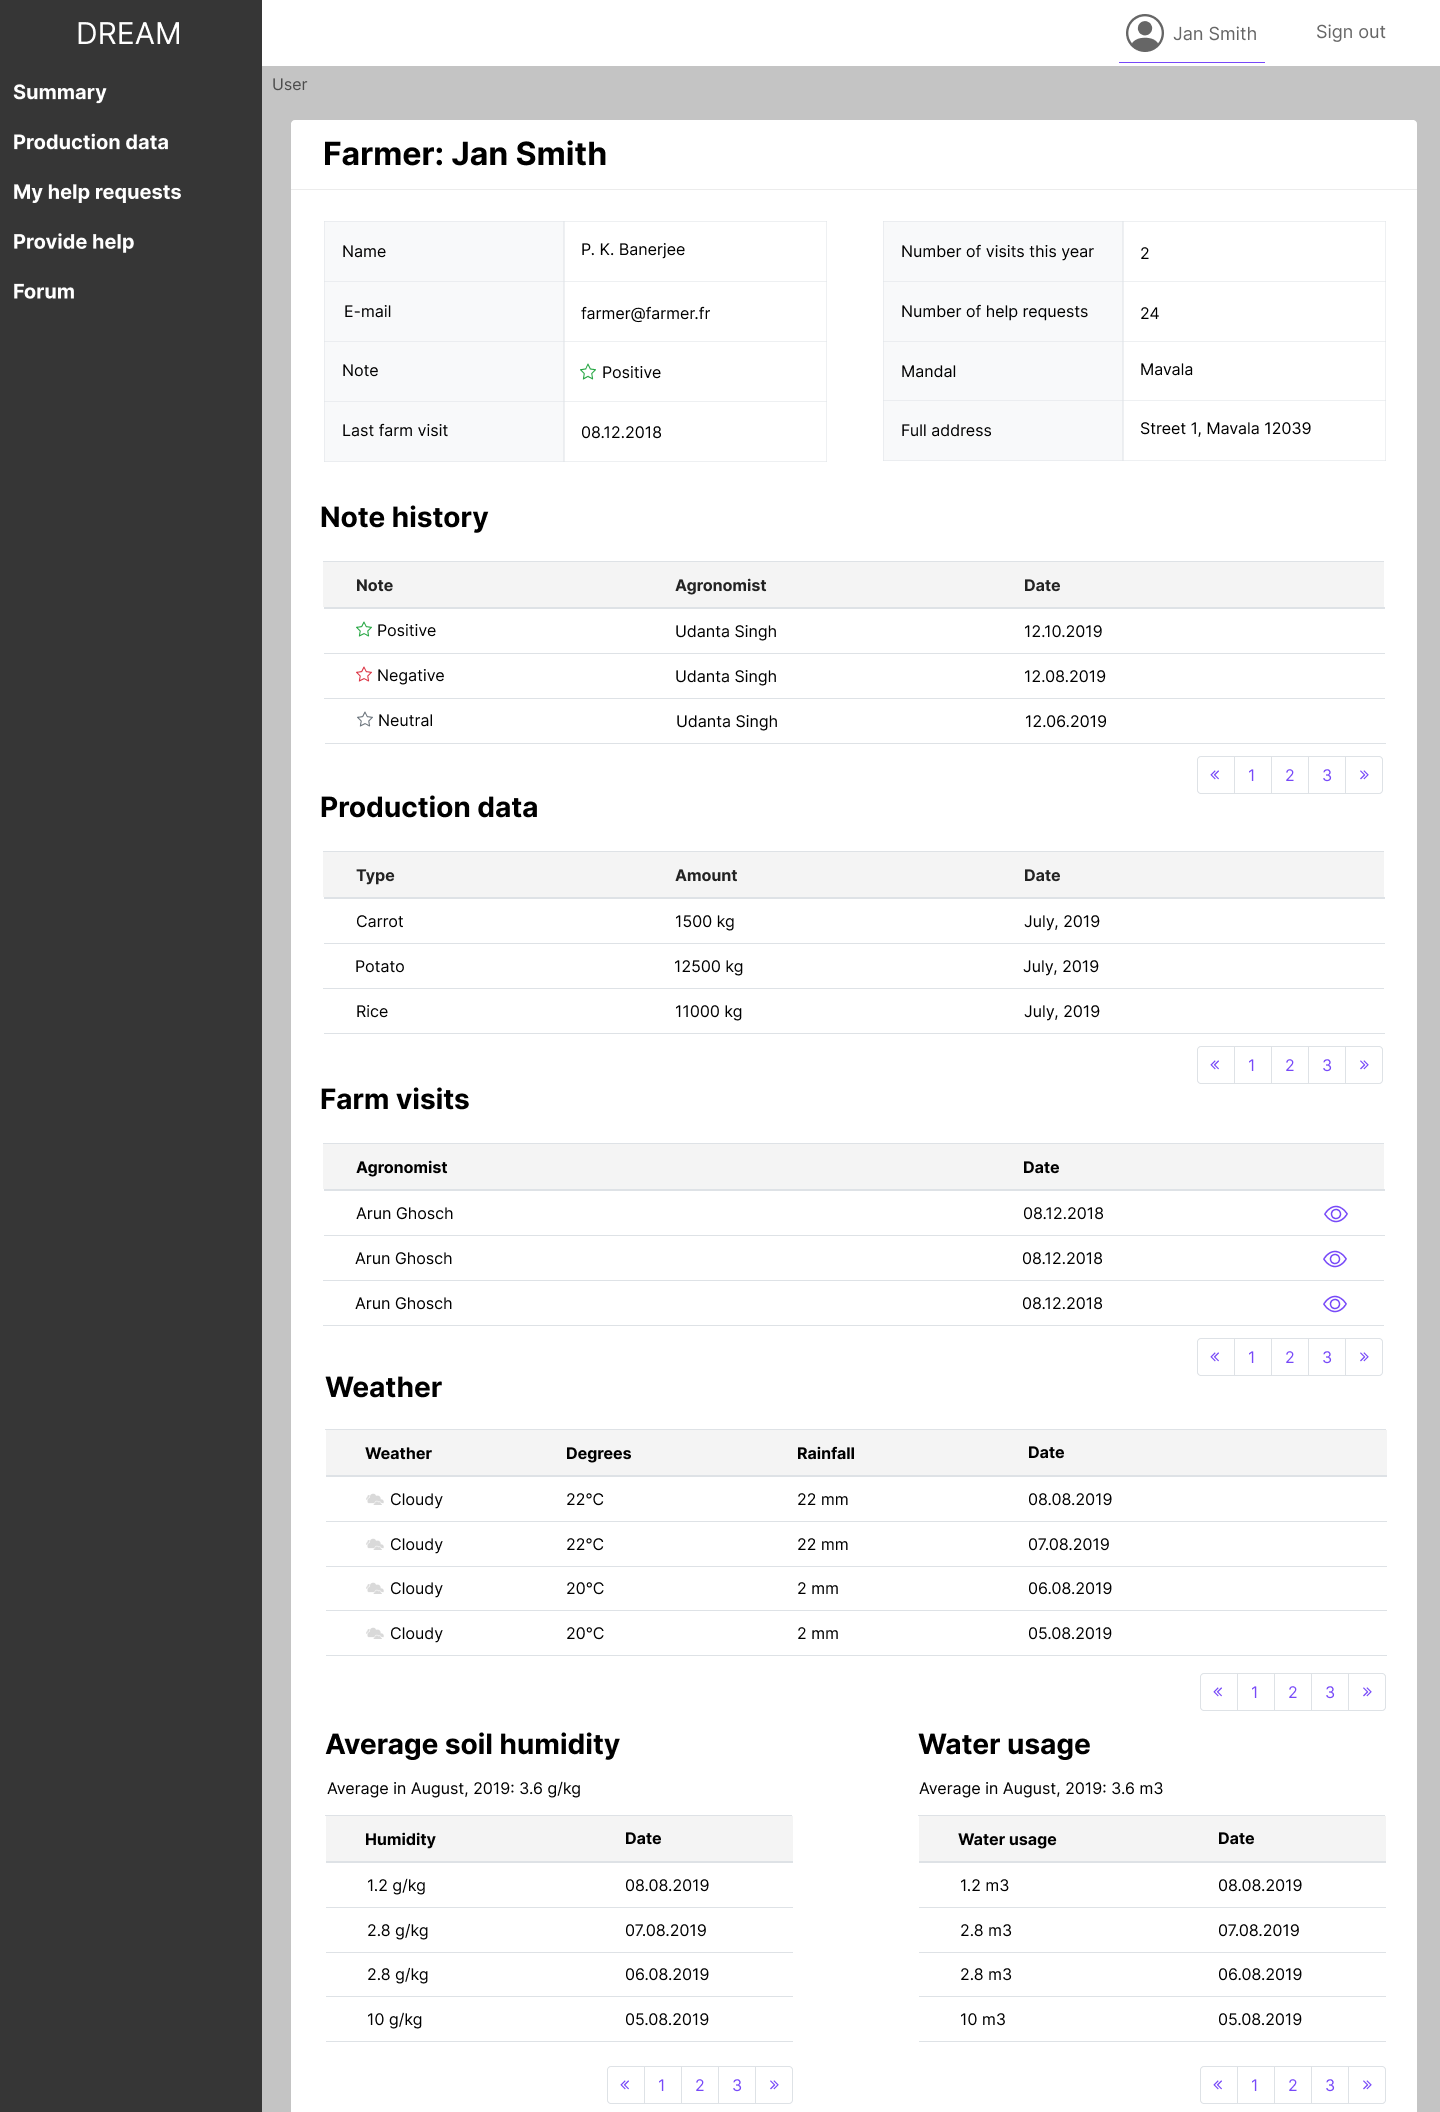
\includegraphics[width=0.75\textwidth]{mockups/Farmer_User_part1.png}
        \caption{\textbf{M6.1.} Farmer's user view - part 1.}
        \label{fig:farmer-summary}
    \end{figure}
    \begin{figure}[H]
        \centering
        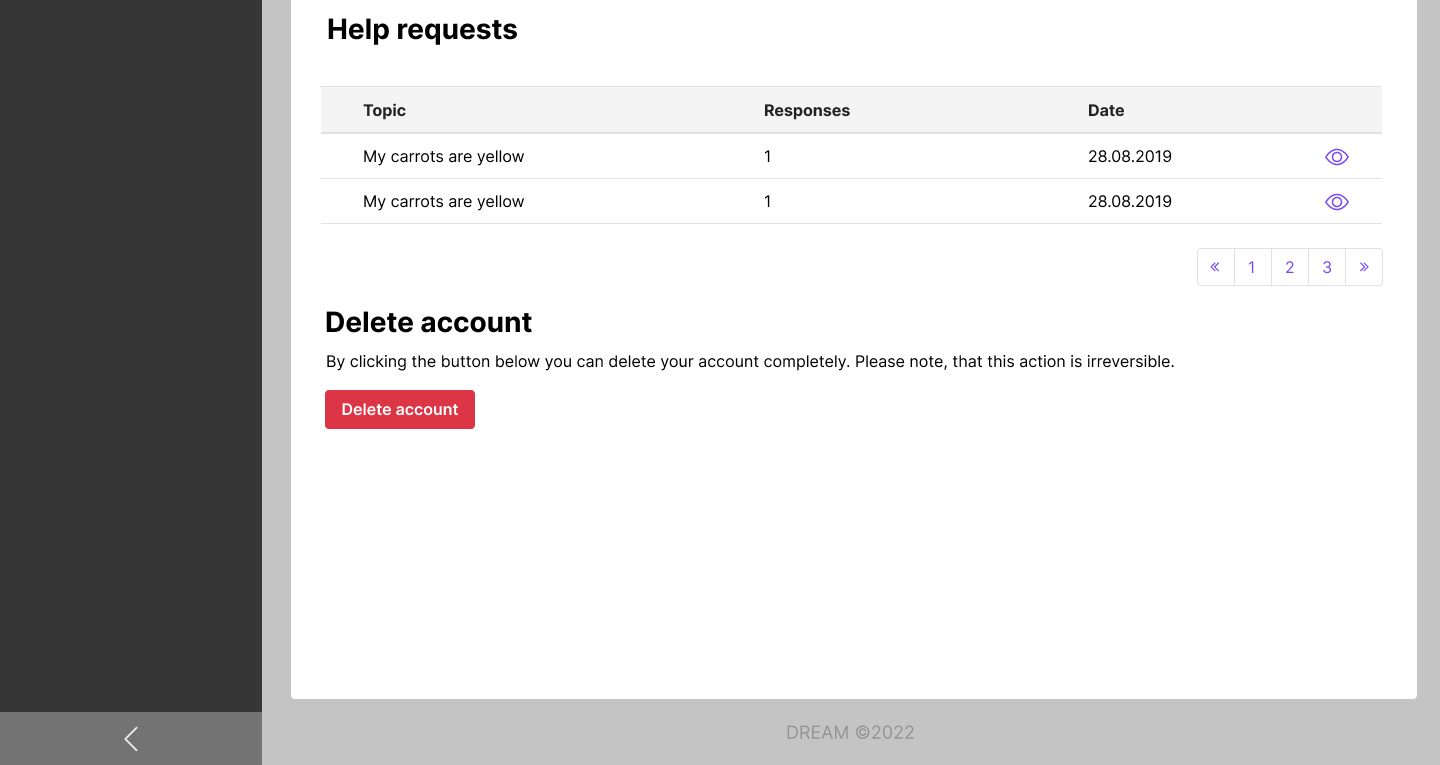
\includegraphics[width=0.75\textwidth]{mockups/Farmer_User_part2.png}
        \caption{\textbf{M6.2.} Farmer's user view - part 2.}
    \end{figure}
    
    Directly after logging in, farmer is forwarded to the dashboard page, containing a summary of the most important information. From there he can navigate to other views by the navigation bar in the left part of the page, the navigation bar in the upper part of the page or by clicking on the button in the lower part of some summary cards.  
    \begin{figure}[H]
        \centering
        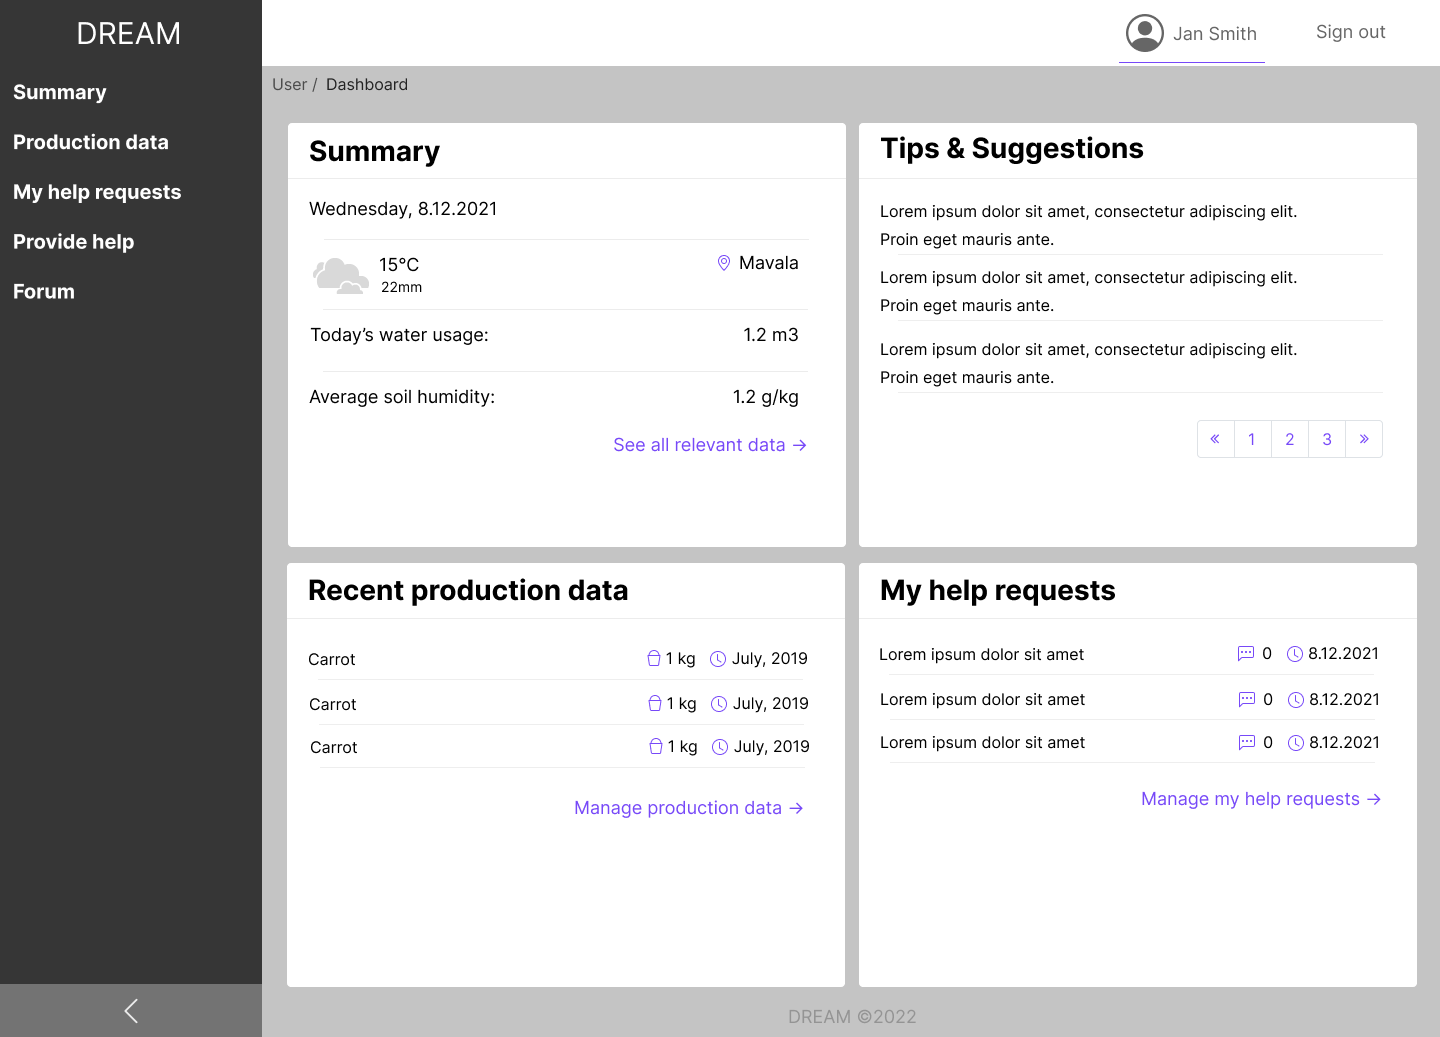
\includegraphics[width=0.75\textwidth]{mockups/Farmer_Dashboard.png}
        \caption{\textbf{M7.} Farmer's dashboard.}
    \end{figure}
    
    The farmer can manage his production data, by choosing the option \textit{Production data} in the left navigation bar. The production data view consists of a table with the latest data, an \textit{Add new} button and an option to delete previously provided information. After clicking on the \textit{Add new} button, a modal dialog appears, allowing the farmer to create a new entry.
    \begin{figure}[H]
        \centering
        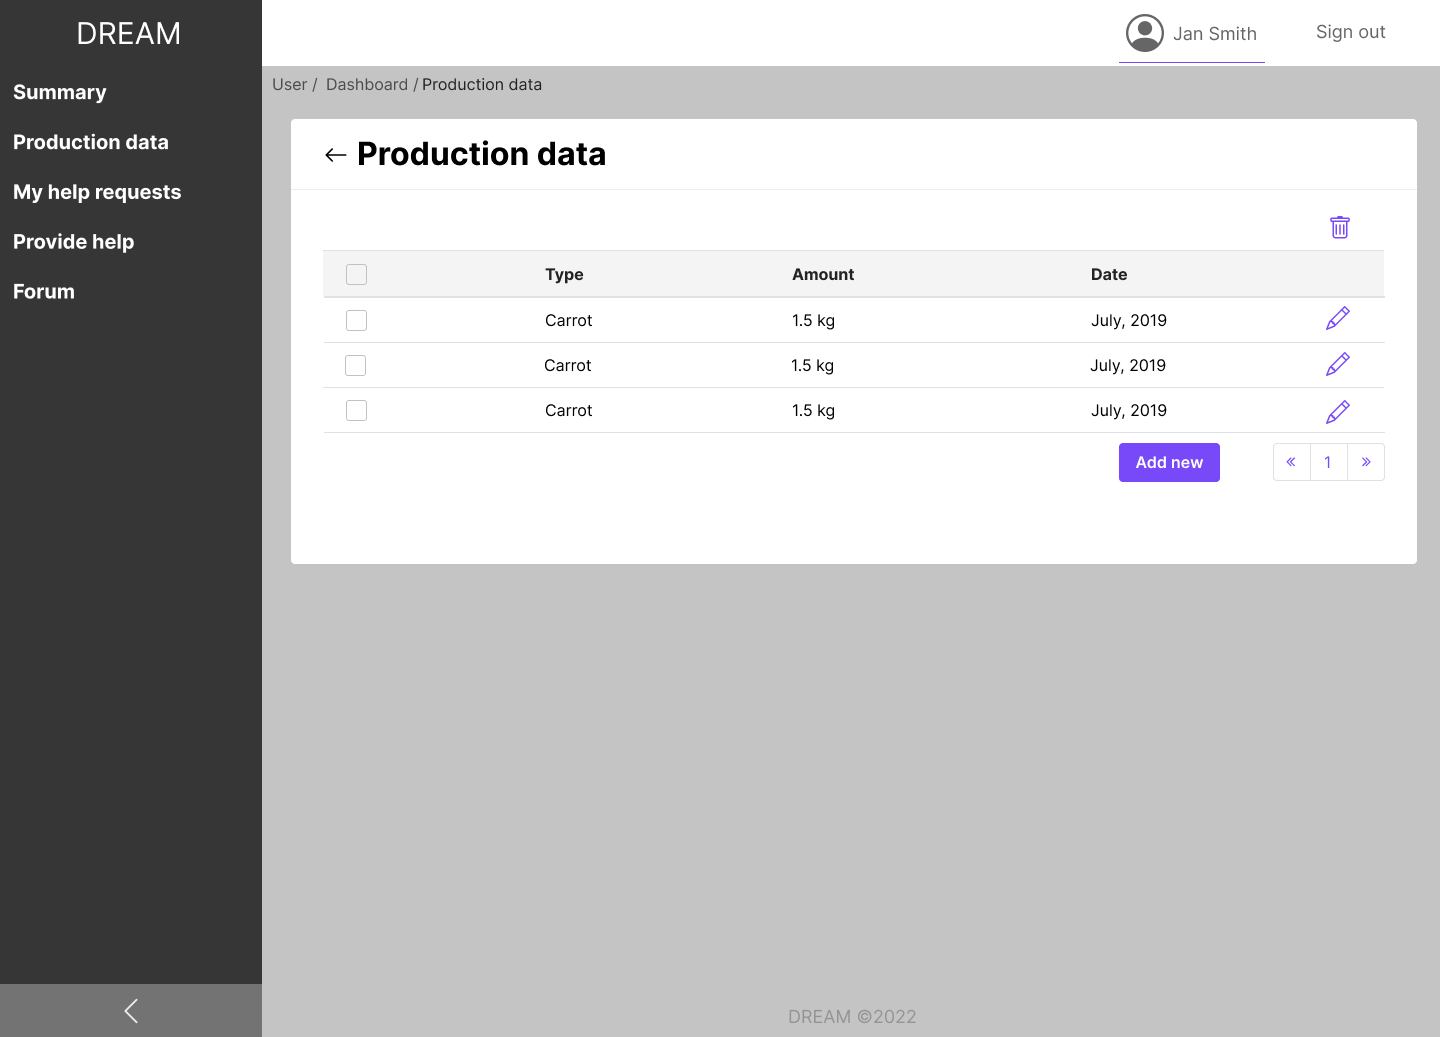
\includegraphics[width=0.75\textwidth]{mockups/Farmer_Dashboard_Production data.png}
        \caption{\textbf{M8.} Farmer's production data.}
    \end{figure}
    
    The farmer can see all his help requests, by clicking on \textit{My help requests} option in the left navigation bar. Help requests are visualized in the form of a table, with entries containing a short summary of given help requests. User can view detailed information by clicking on given entry or create a new help requests, by clicking on \textit{Create help request} button. The farmer can also search for a help requests by topic, using a search bar in the upper part of the content card.
    \begin{figure}[H]
        \centering
        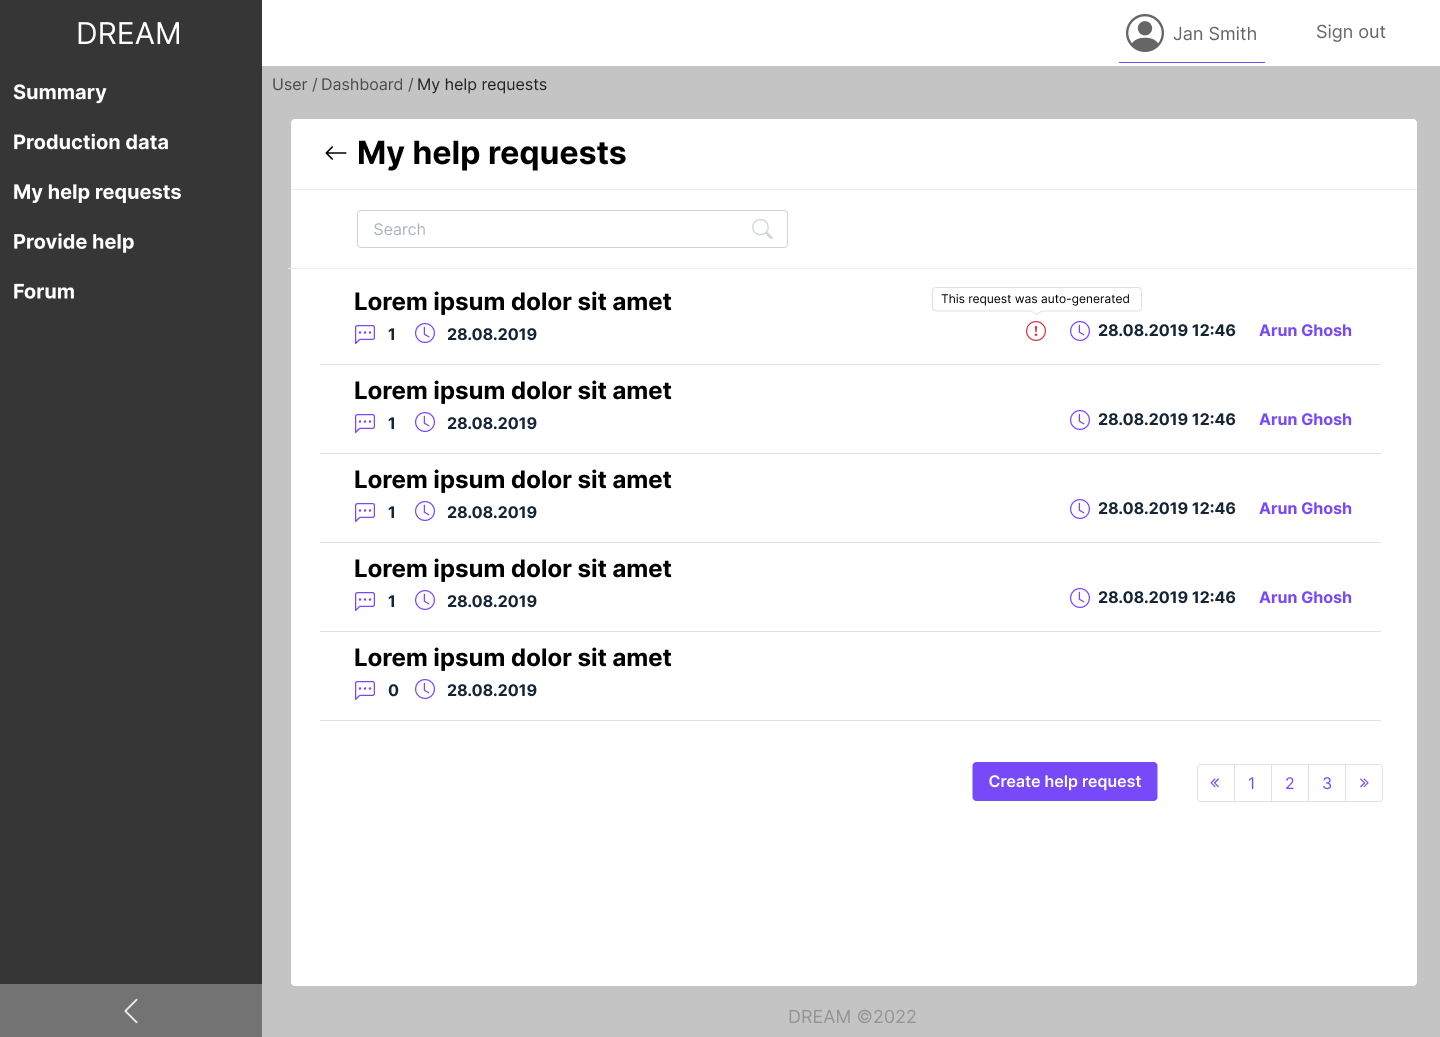
\includegraphics[width=0.75\textwidth]{mockups/Farmer_Dashboard_My help requests.png}
        \caption{\textbf{M9.} Help requests created by farmer.}
    \end{figure}
    
    After clicking on a given entry in the help request table, the user is redirected to a view, containing all detailed information about the help requests, as well as advice provided by other farmers and agronomists.
    \begin{figure}[H]
        \centering
        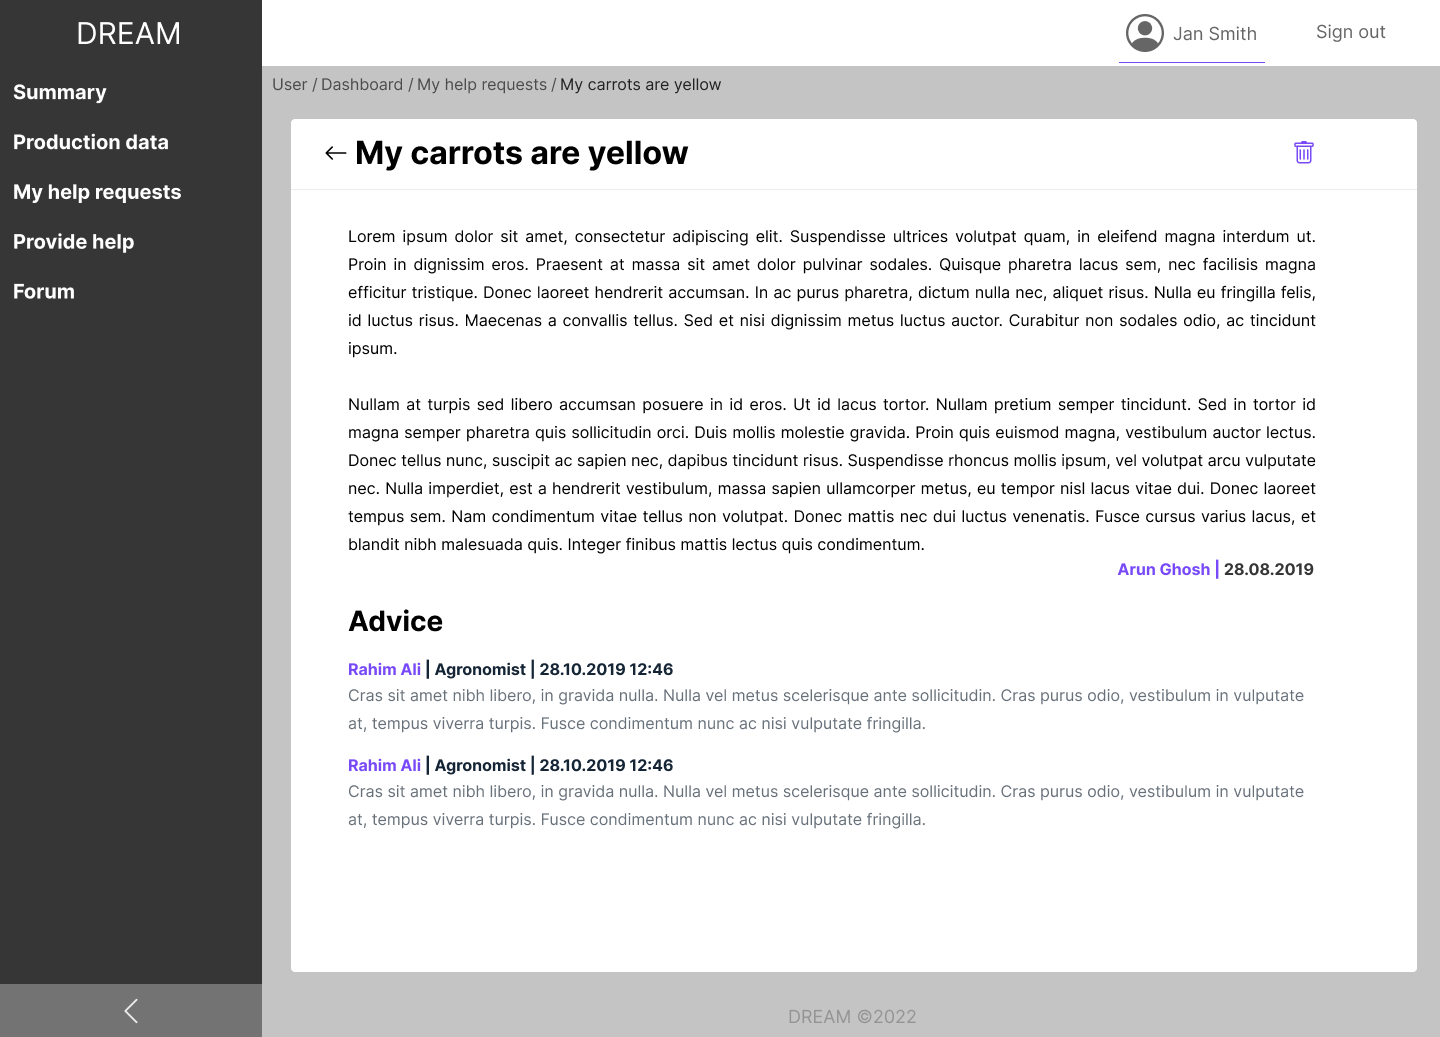
\includegraphics[width=0.75\textwidth]{mockups/Farmer_Dashboard_My help requests_VIew request.png}
        \caption{\textbf{M10.} Specific help request created by farmer.}
    \end{figure}
    
    After clicking on the \textit{Create help request} button in the help requests view, a modal dialog appears, allowing the farmer to create a new help request, by filling in the topic and message.
    \begin{figure}[H]
        \centering
        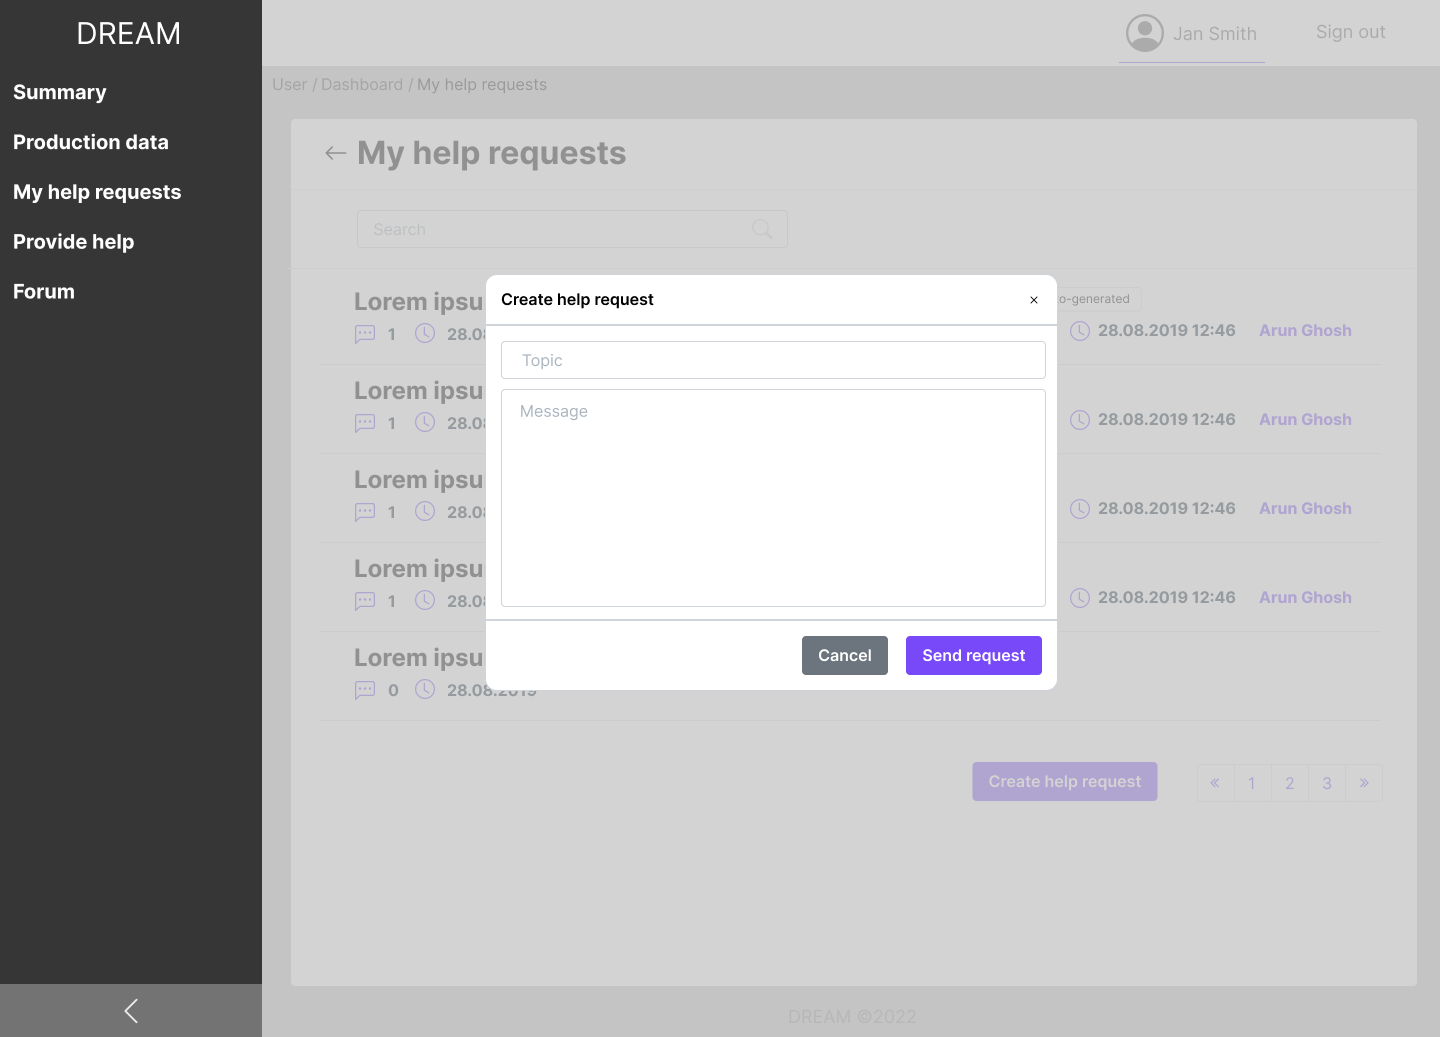
\includegraphics[width=0.75\textwidth]{mockups/Farmer_Dashboard_My help requests_Create help request.png}
        \caption{\textbf{M11.} Creating help request.}
    \end{figure}
    
    The farmer with positive note can see all received help requests, by clicking on \textit{Provide help} option in the left navigation bar. Help requests are visualized in the form of a table, with entries containing a short summary of given help requests. User can view detailed information by clicking on a given entry. The farmer can search for a help requests by topic, using a search bar in the upper part of the content card.
    \begin{figure}[H]
        \centering
        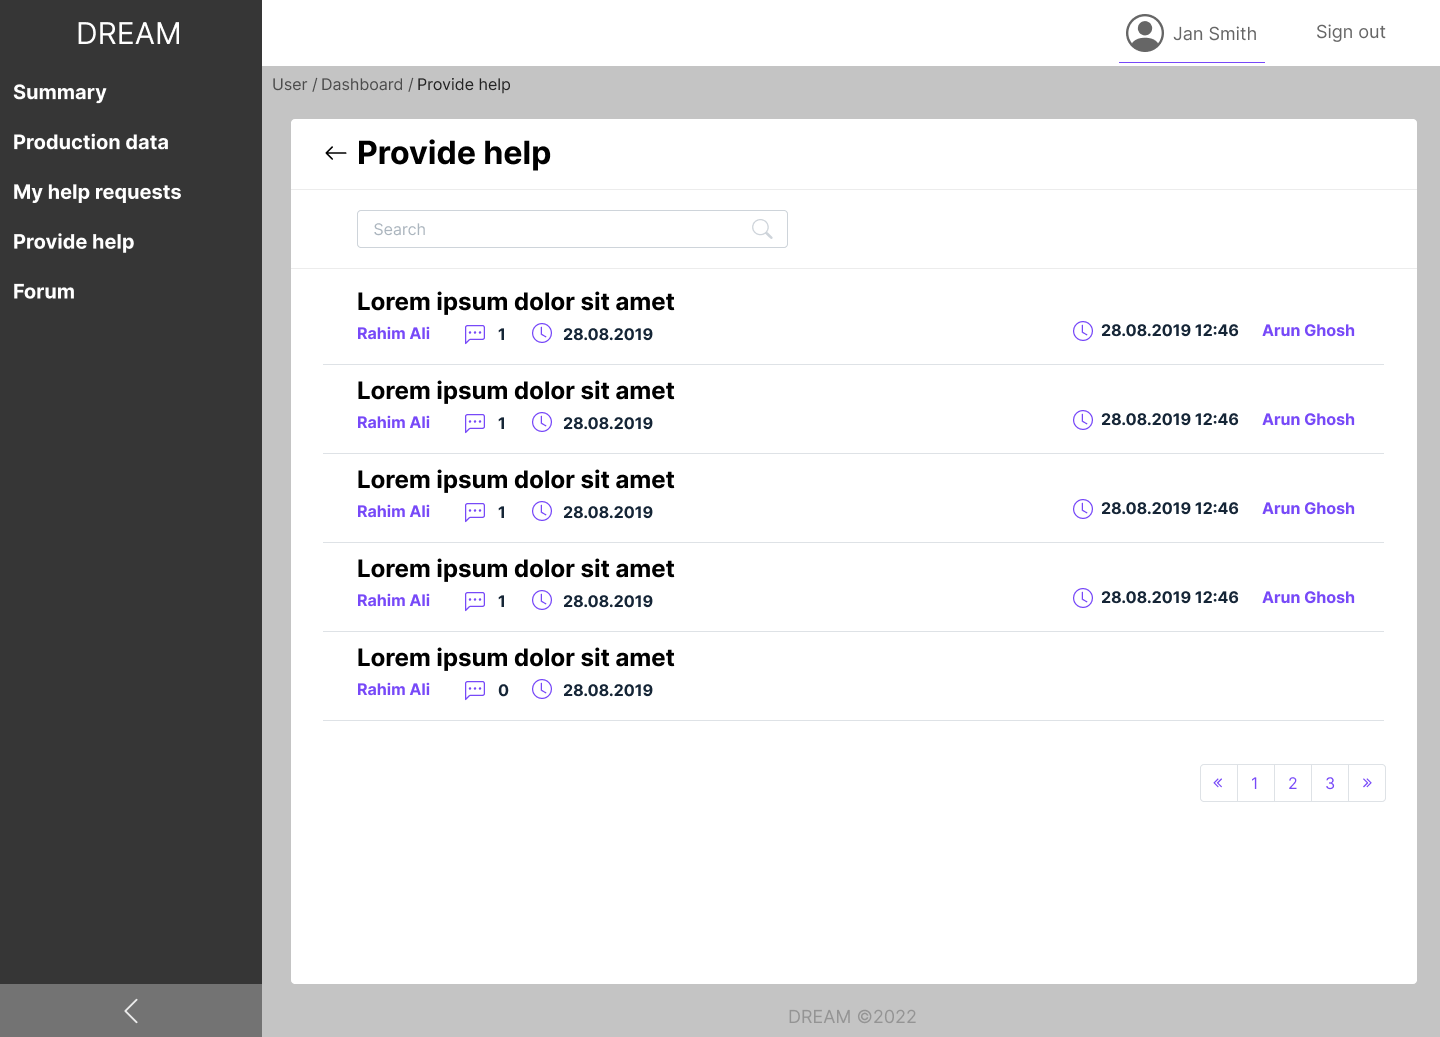
\includegraphics[width=0.75\textwidth]{mockups/Farmer_Dashboard_Provide help.png}
        \caption{\textbf{M12.} Help requests received by farmer with positive note.}
        \label{fig:farmer-provide-help}
    \end{figure}
    
    
    After clicking on a given entry in the help request table, the user is redirected to a view, containing all detailed information about the help requests and allowing the farmer to create a new advice, by filling a short form on the bottom of the page. This view is also accessible for agronomists, by clicking on the \textit{Provide help} button in agronomist's left navigation bar.
    \begin{figure}[H]
        \centering
        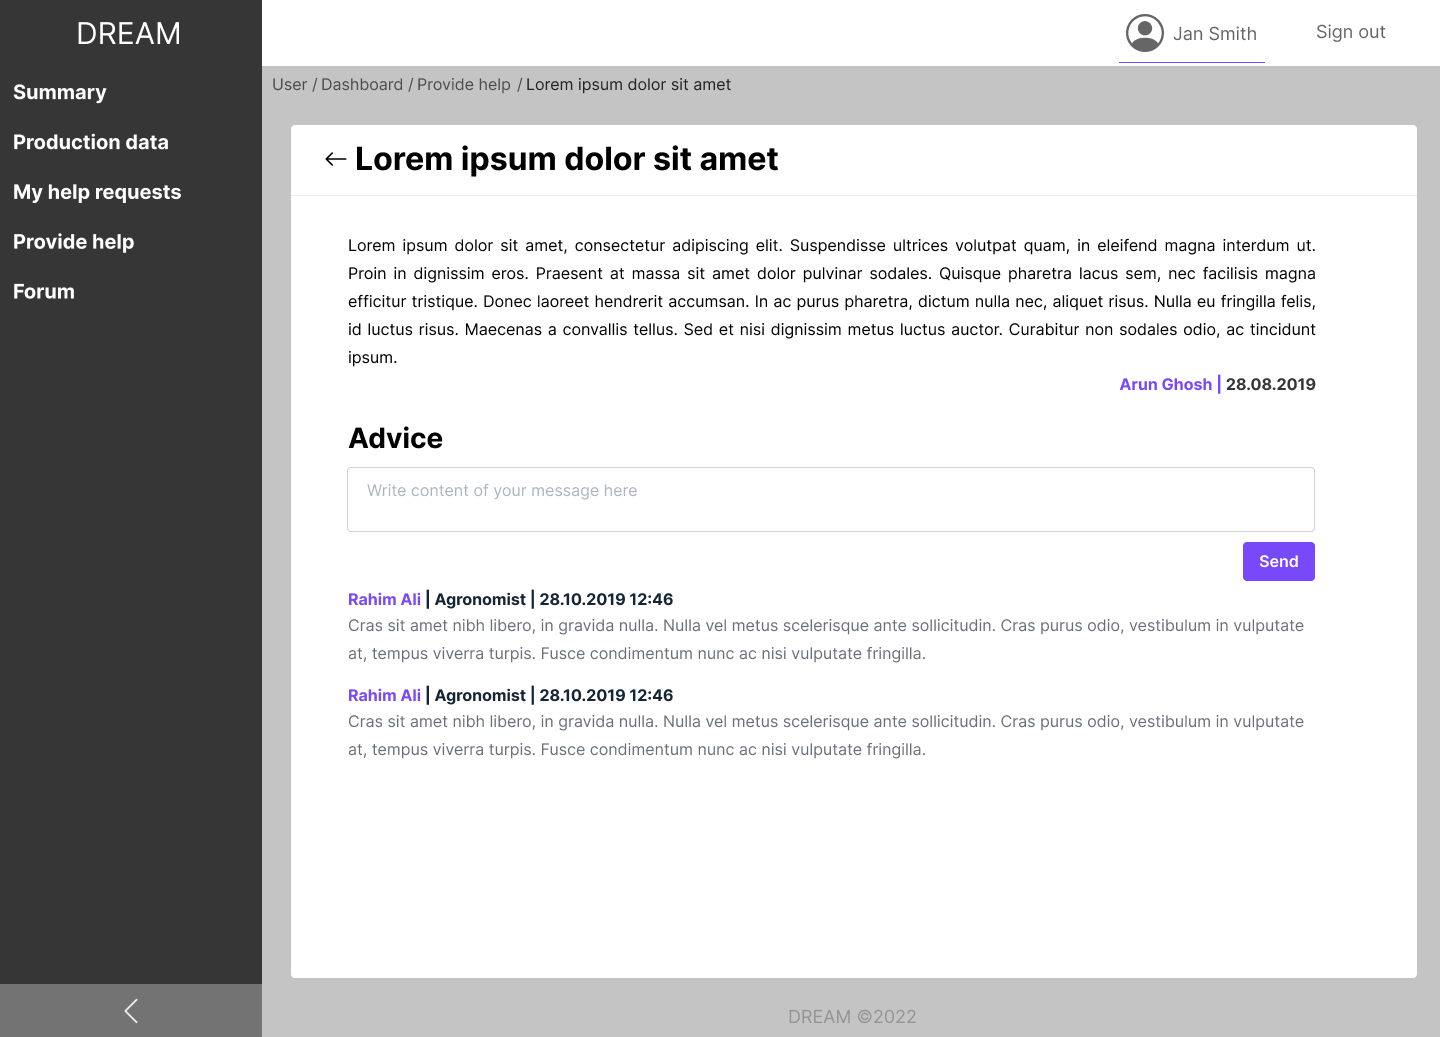
\includegraphics[width=0.75\textwidth]{mockups/Farmer_Dashboard_Provide help_Request.png}
        \caption{\textbf{M13.} Specific help request received by farmer with positive note (applicable also for the agronomist).}
    \end{figure}
    
    The farmer can access the forum using \textit{Forum} button in the left navigation bar. The forum is built similarly to the help requests view – it consists of a table, with entries showing a short summary of a given thread. The user can search for a thread by name using the search bar, located in the upper part of the content card, display a detailed thread view, by clicking on the entry or create a new forum thread, using the \textit{Create forum thread} button in the lower part of the content card.
    \begin{figure}[H]
        \centering
        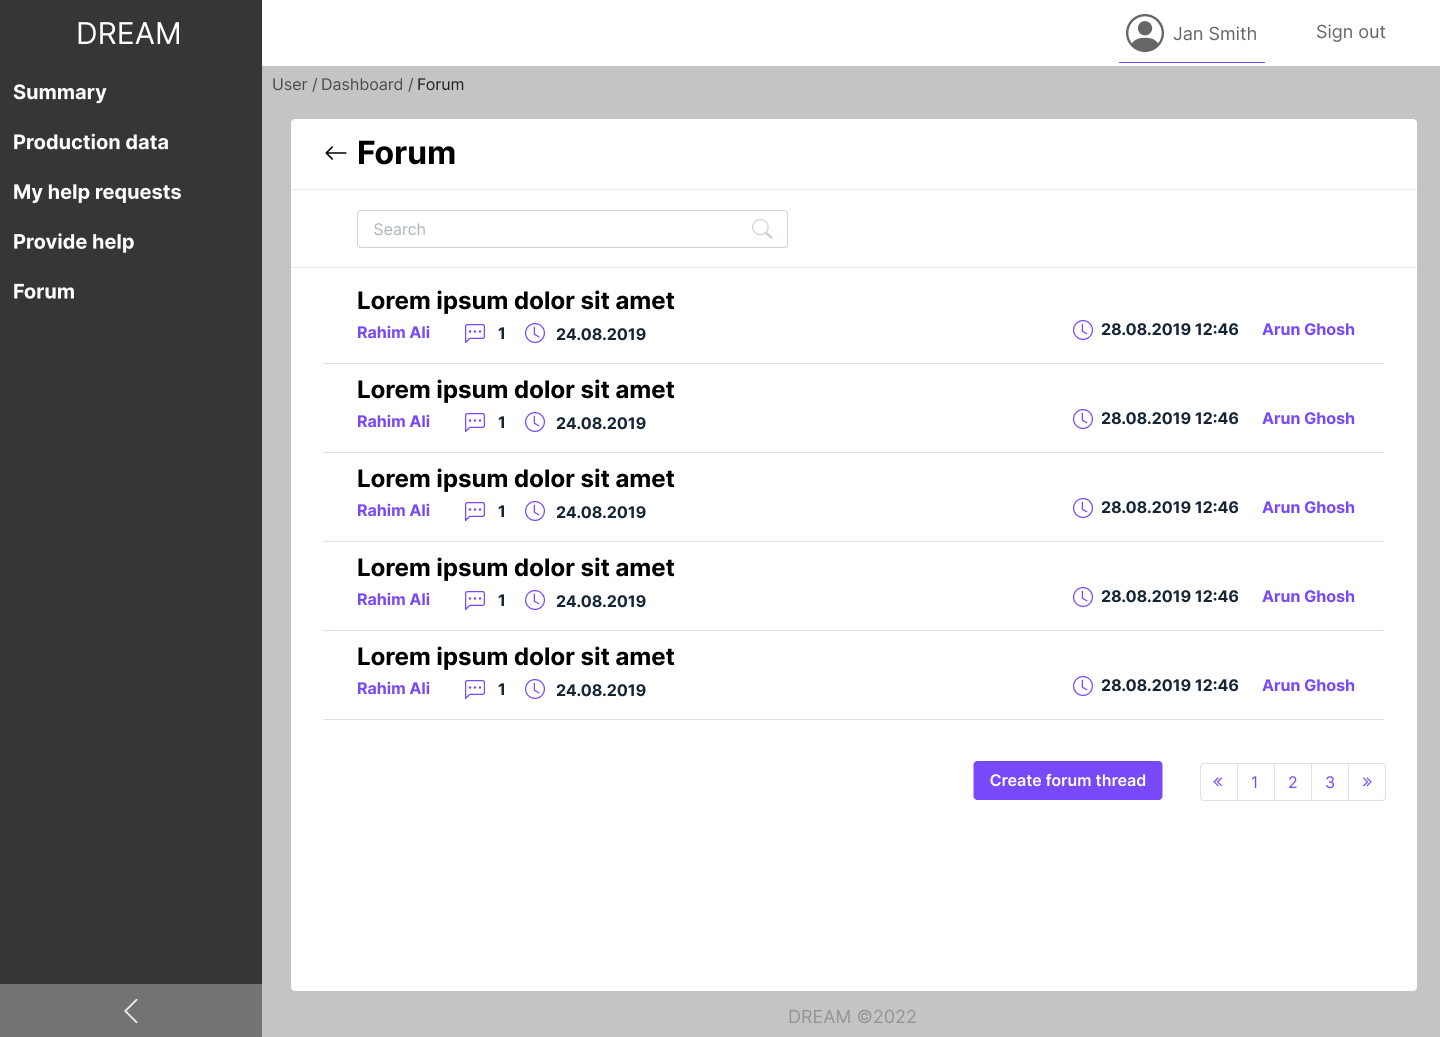
\includegraphics[width=0.75\textwidth]{mockups/Farmer_Dashboard_Forum.png}
        \caption{\textbf{M14.} Forum view.}
    \end{figure}
    
    After clicking on a given entry in the forum thread table, the farmer is redirected to a detailed thread view. The user can create a comment, by filling a short form in the lower part of the content card or delete a previously created comment, using the thrash icon next to the entry.
    \begin{figure}[H]
        \centering
        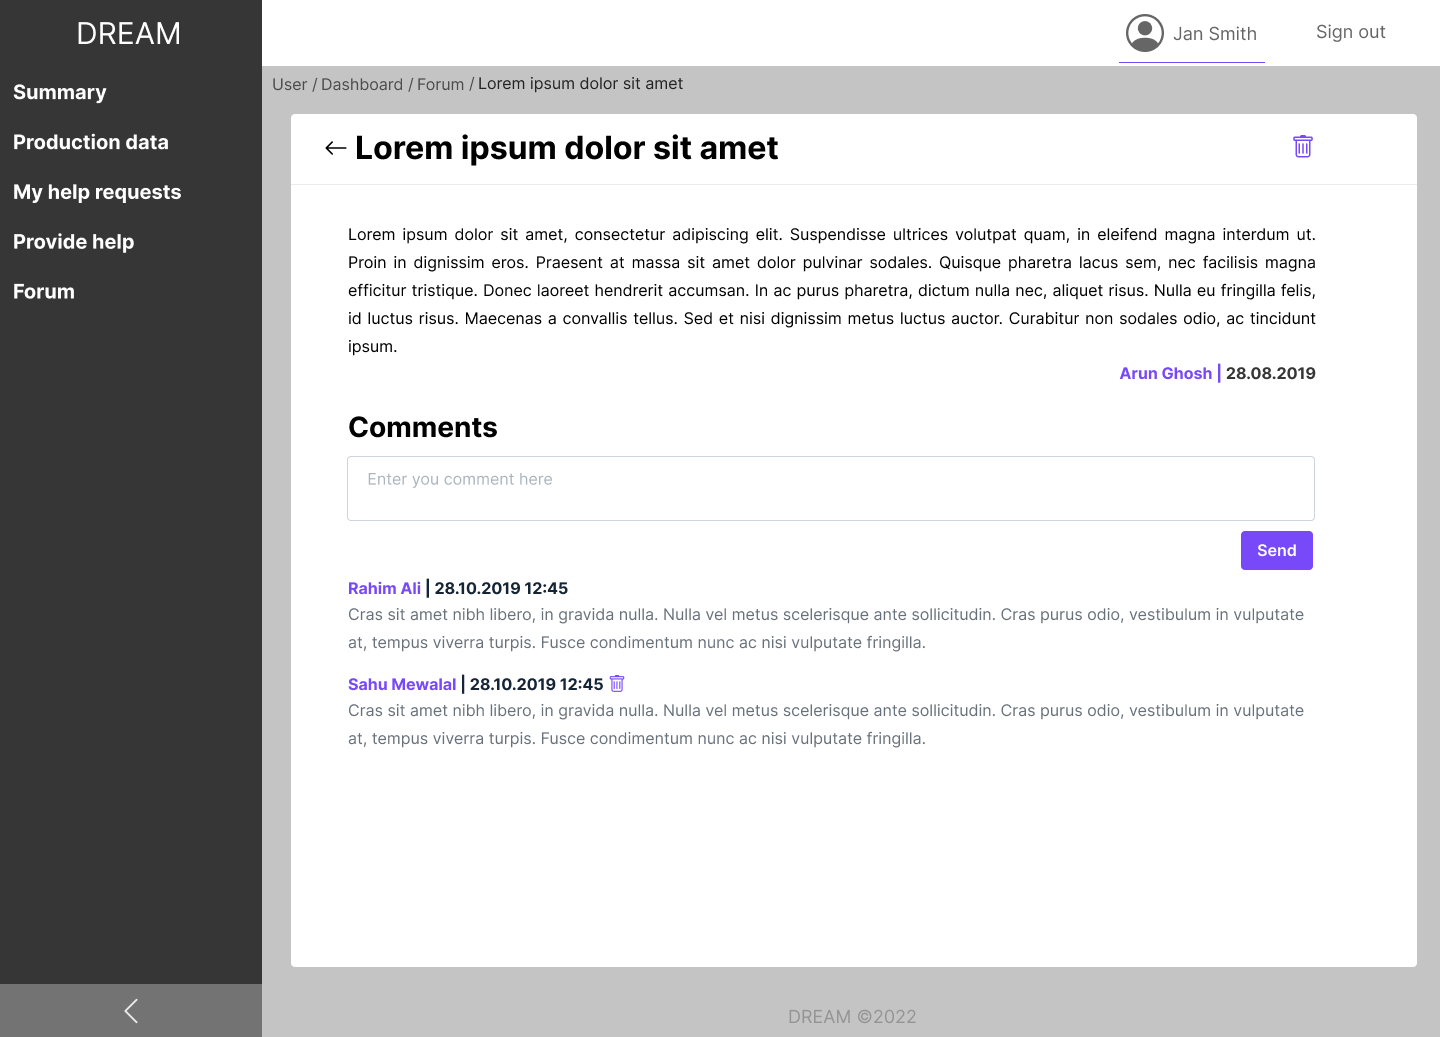
\includegraphics[width=0.75\textwidth]{mockups/Farmer_Dashboard_Forum_Thread.png}
        \caption{\textbf{M15.} Specific forum thread.}
    \end{figure}
    
    After clicking on the \textit{Create forum thread} button in the help requests view, a modal dialog appears, allowing the farmer to create a new forum thread, by filling topic and message.
    \begin{figure}[H]
        \centering
        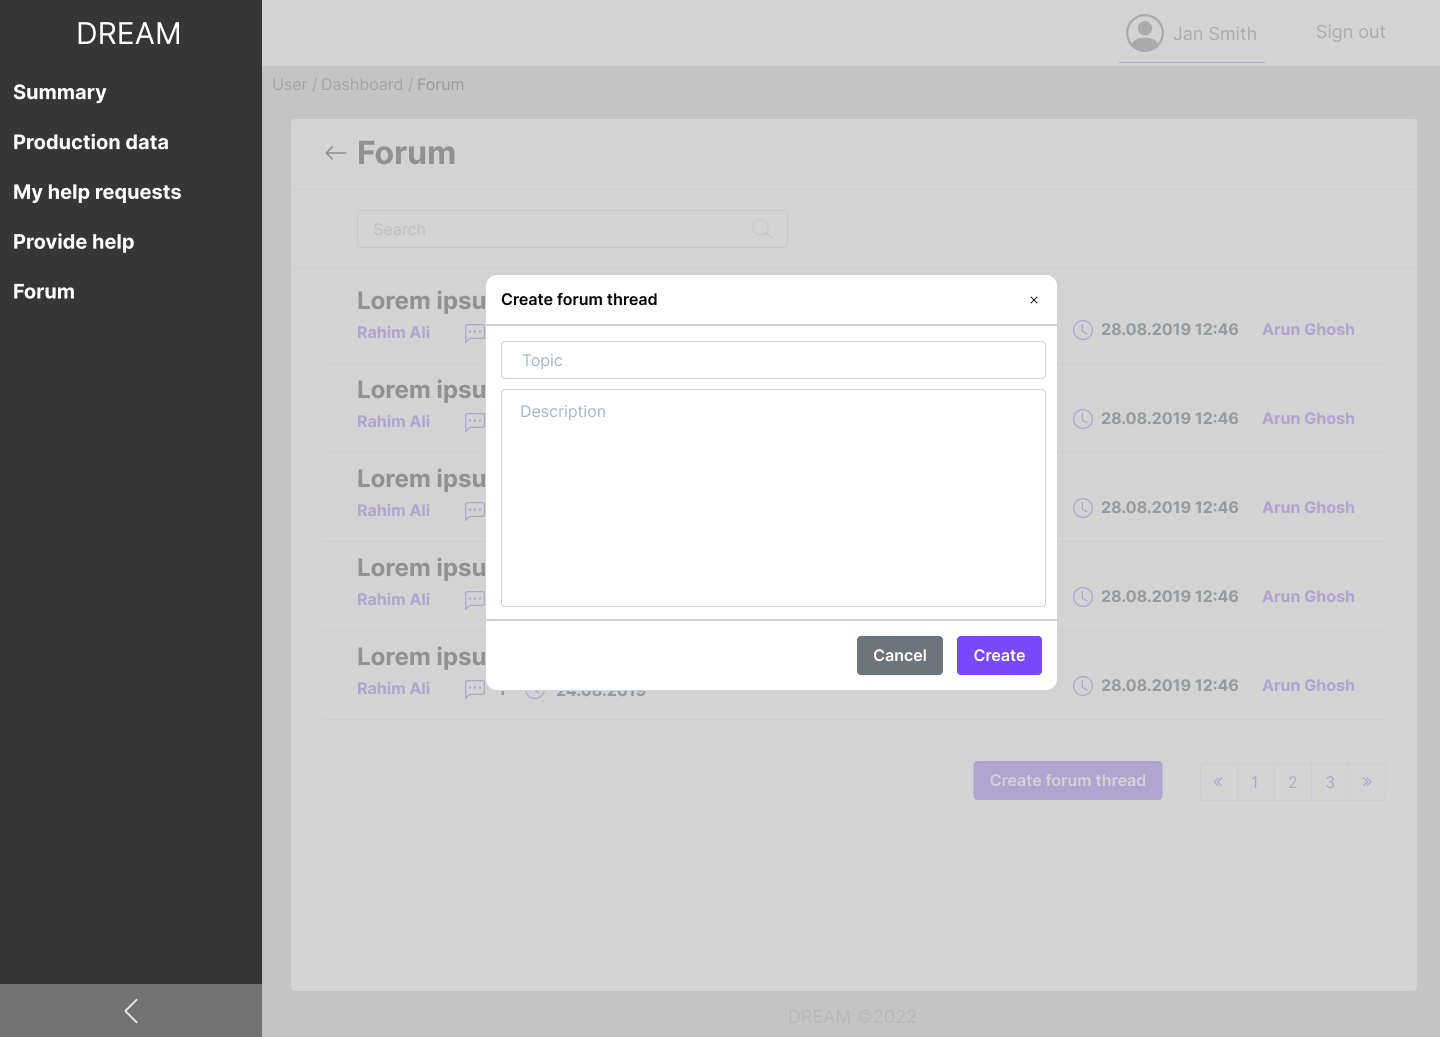
\includegraphics[width=0.75\textwidth]{mockups/Farmer_Dashboard_Forum_Create thread.png}
        \caption{\textbf{M16.} Creating forum thread.}
    \end{figure}
    
    
    \subsubsection{Agronomist}
    
    The agronomist can open his account summary, by clicking on the button in the top navigation bar, containing his name and surname. In the user view, he can view his account details, manage his area of responsibility and delete his account.
    \begin{figure}[H]
        \centering
        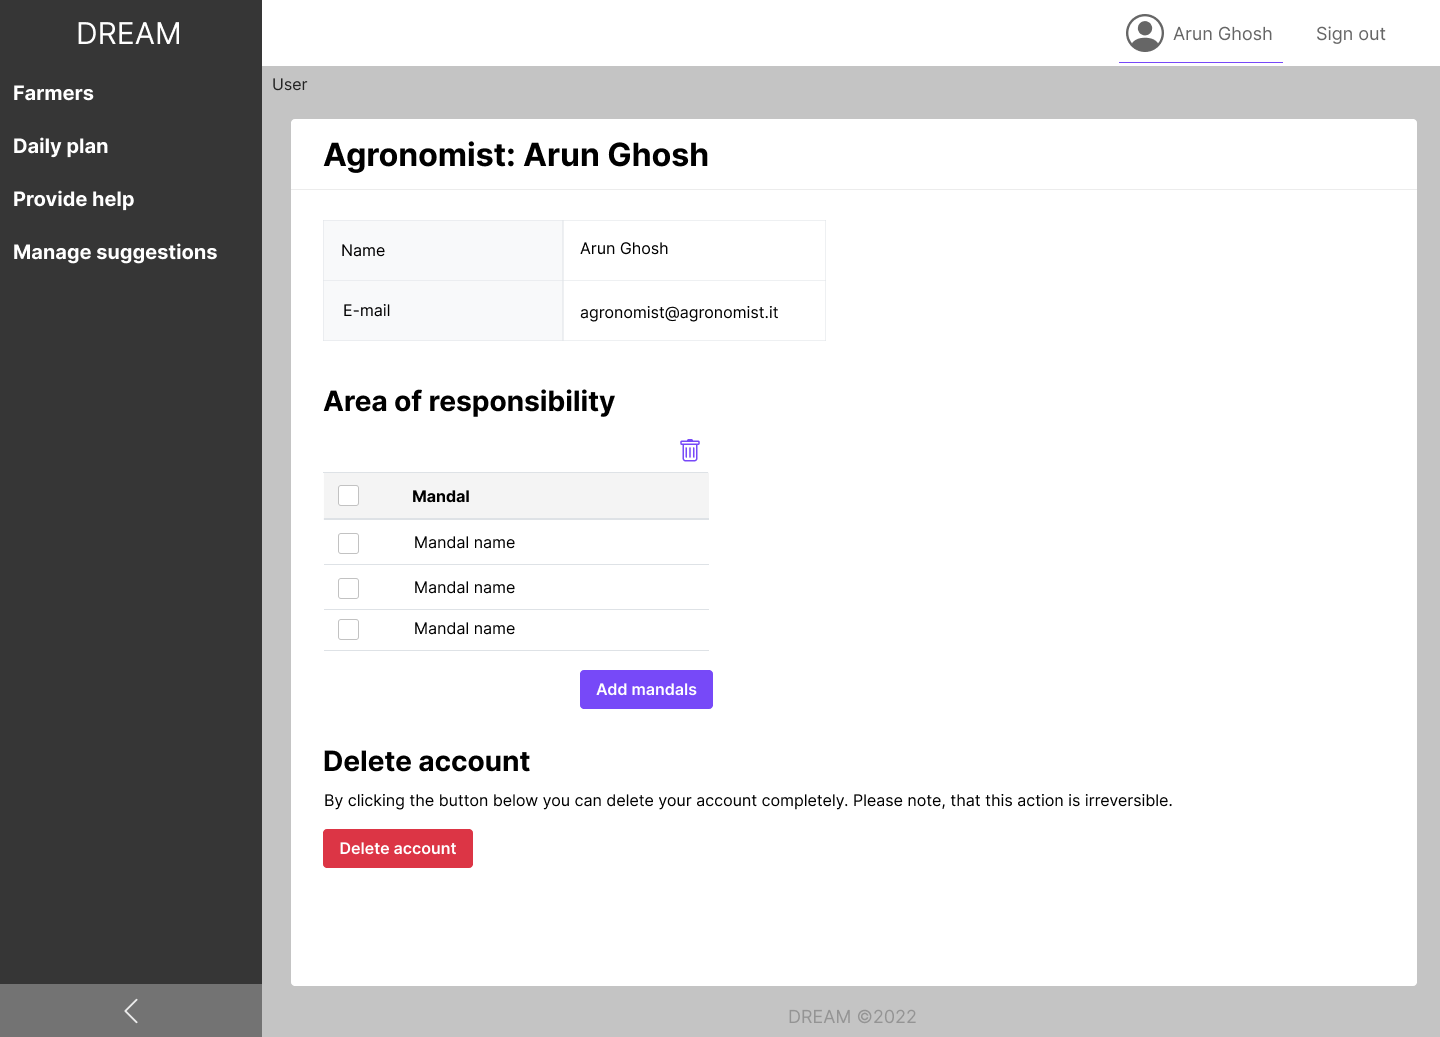
\includegraphics[width=0.75\textwidth]{mockups/Agronomist_User.png}
        \caption{\textbf{M17.} Agronomist's user view.}
    \end{figure}
    
    Directly after logging in, an agronomist is redirected to the dashboard view, which contains a summary of the most important information, such as a short list of farmer in his area of responsibility, today’s visits and last help requests received. He can navigate to other views using the left and top navigation bar or detailed button in the lower part of the content cards.
    \begin{figure}[H]
        \centering
        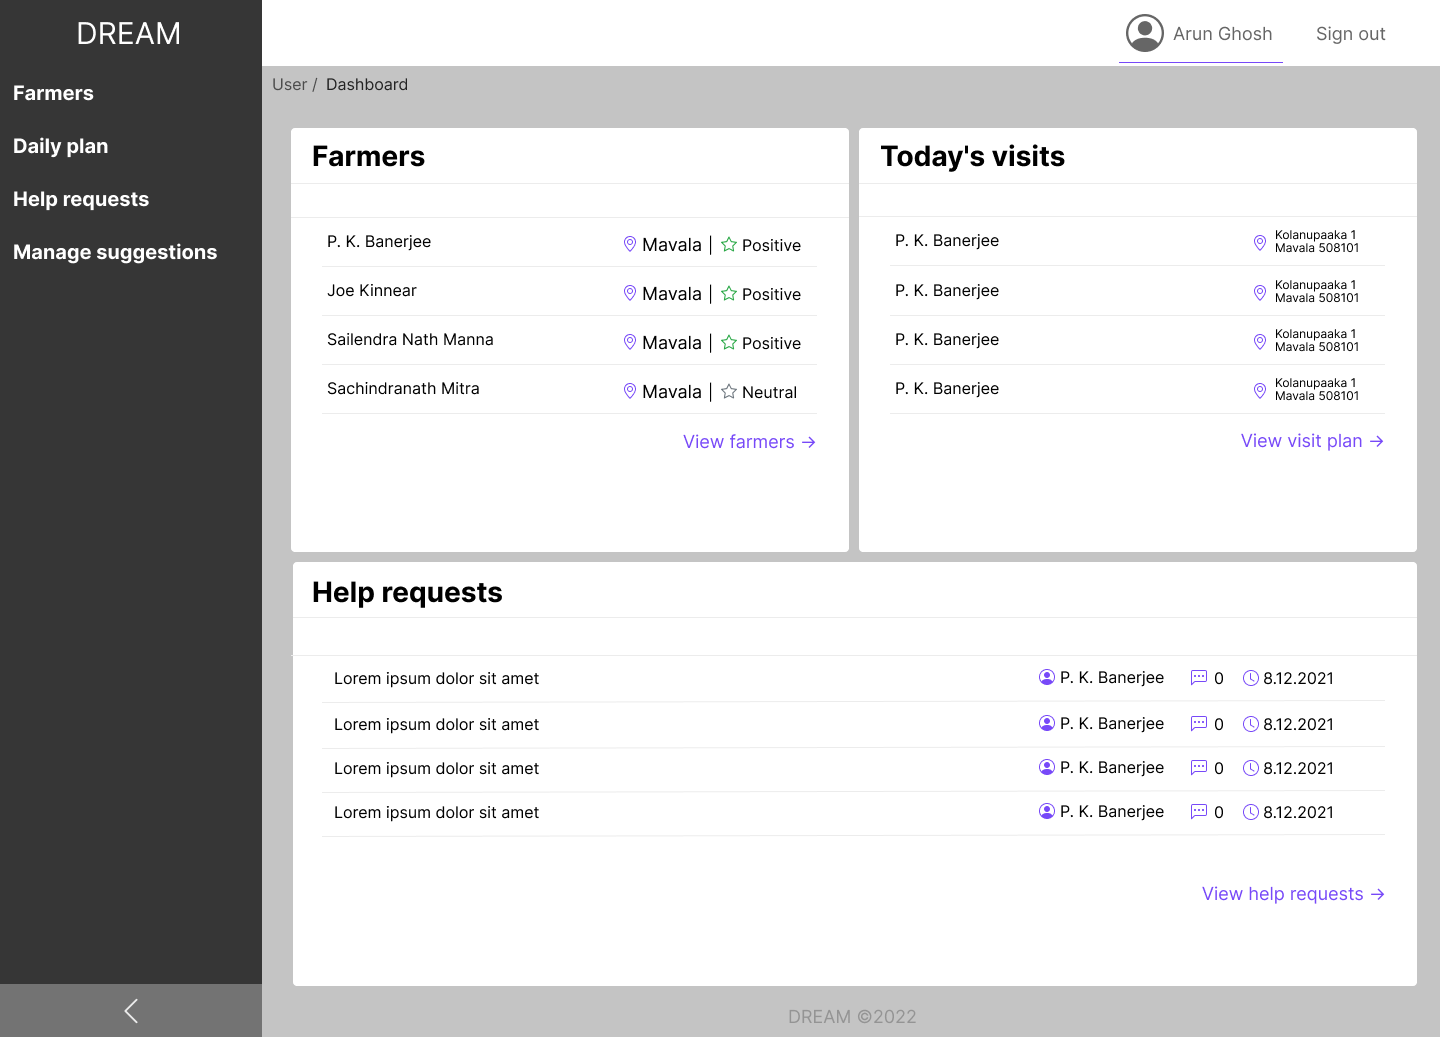
\includegraphics[width=0.75\textwidth]{mockups/Agronomist_Dashboard.png}
        \caption{\textbf{M18.} Agronomist's dashboard.}
    \end{figure}
    
    The agronomist can display a list of farmers in his area of responsibility, using the \textit{Farmer} option in the left navigation bar. The list consists of a table with entries, presenting the most important information about a farmer, as well as a filter bar, allowing the user to search by farmer's name, mandal or note. By clicking on an entry, the user can view a farmer summary analogical to the one available for farmer. This view is identical to the one available for policy maker, using the \textit{Farmer} option in the left navigation bar. The only difference is that policy maker's view contains a list of all farmers in Telangana.
    \begin{figure}[H]
        \centering
        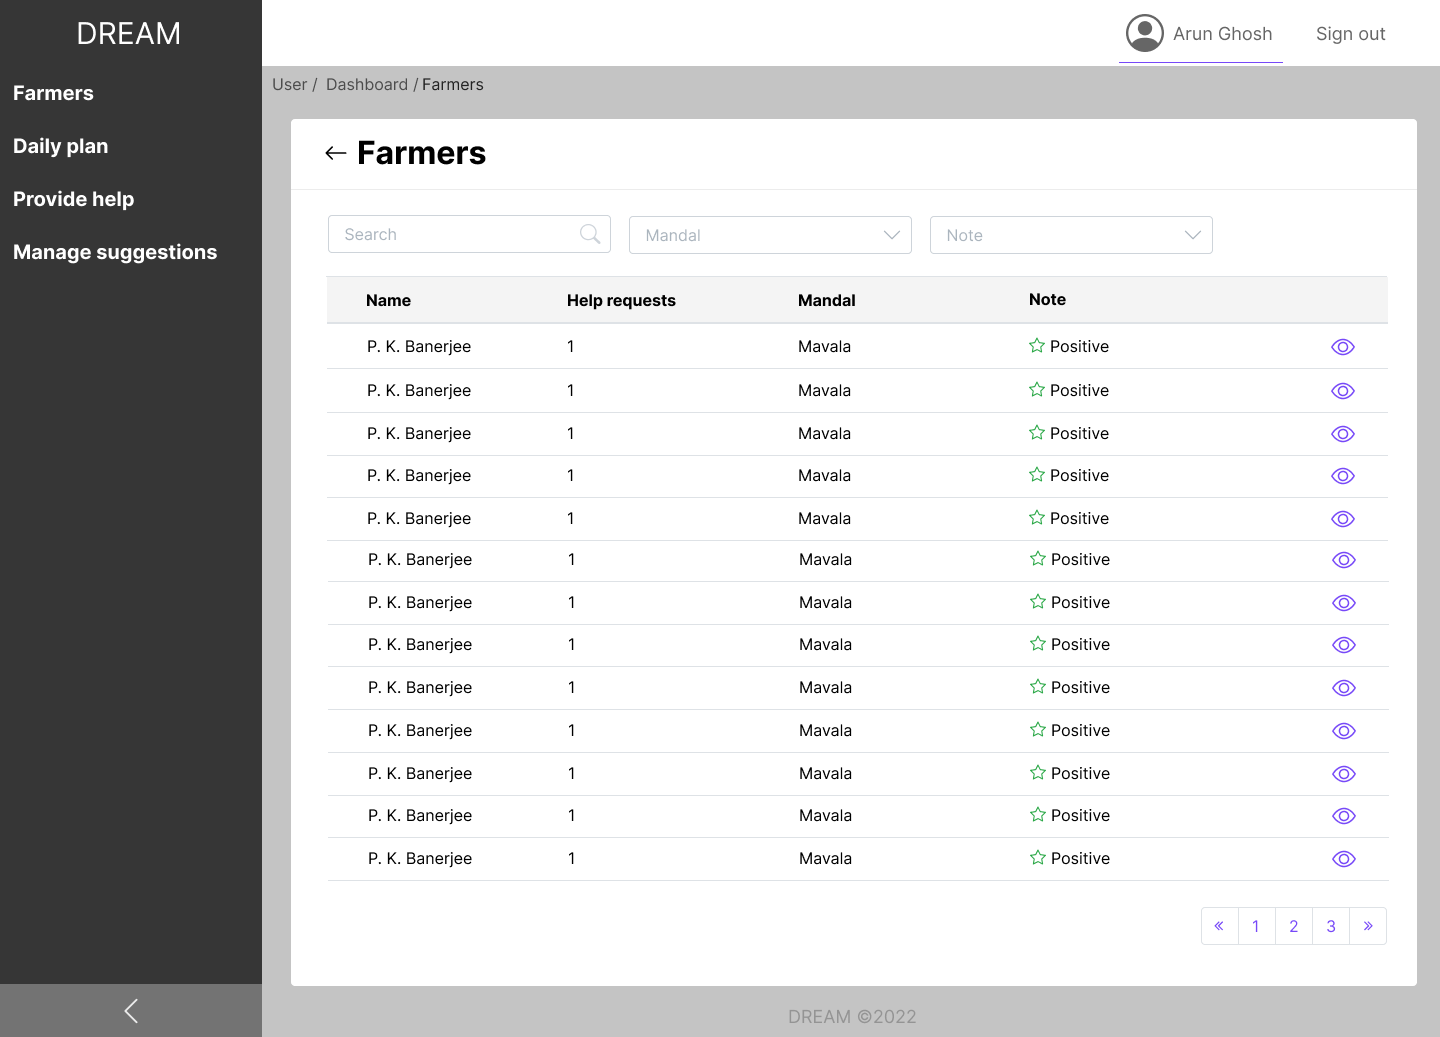
\includegraphics[width=0.75\textwidth]{mockups/Agronomist_Dashboard_Farmers.png}
        \caption{\textbf{M19.} List of farmers (applicable also for the policy maker).}
        \label{fig:agronomist-farmer-list}
    \end{figure}
    
    By clicking on the \textit{Daily plan} button, the agronomist can display his visit calendar and plan for the chosen day. The agronomist can see if he has submitted execution state for the given day: if the day has a green dot on the calendar, it means that the agronomist has realized all his planned visits. A red dot means, that the plan has been submitted, but not all visits were realized. No dot means, that the plan hasn't been submitted yet. The user can manage future visits according to the requirements, using edit and delete buttons next to the given visit. The user can also plan future visits, by clicking on the add button in the upper part of the daily plan.
    
    The described functionality is presented on two following mock-ups: first one shows today/a day in the past, and the next one a day in the future.
    \begin{figure}[H]
        \centering
        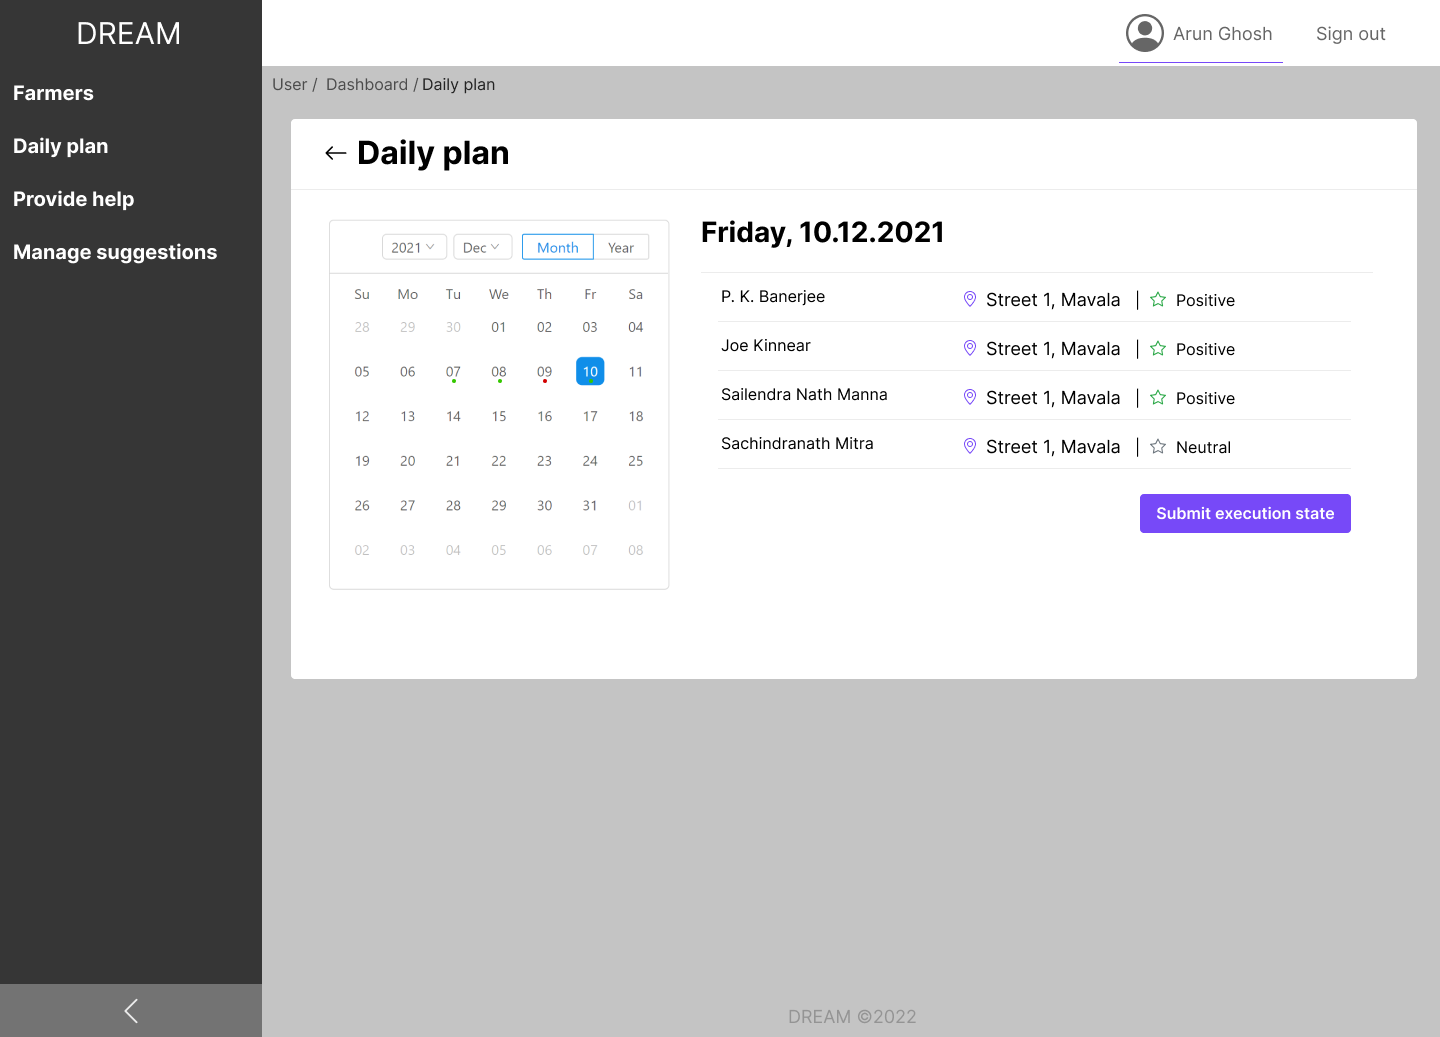
\includegraphics[width=0.75\textwidth]{mockups/Agronomist_Dashboard_Visit plan.png}
        \caption{\textbf{M20.} Calendar of daily plans – view of today or day in the past.}
    \end{figure}
    
    \begin{figure}[H]
        \centering
        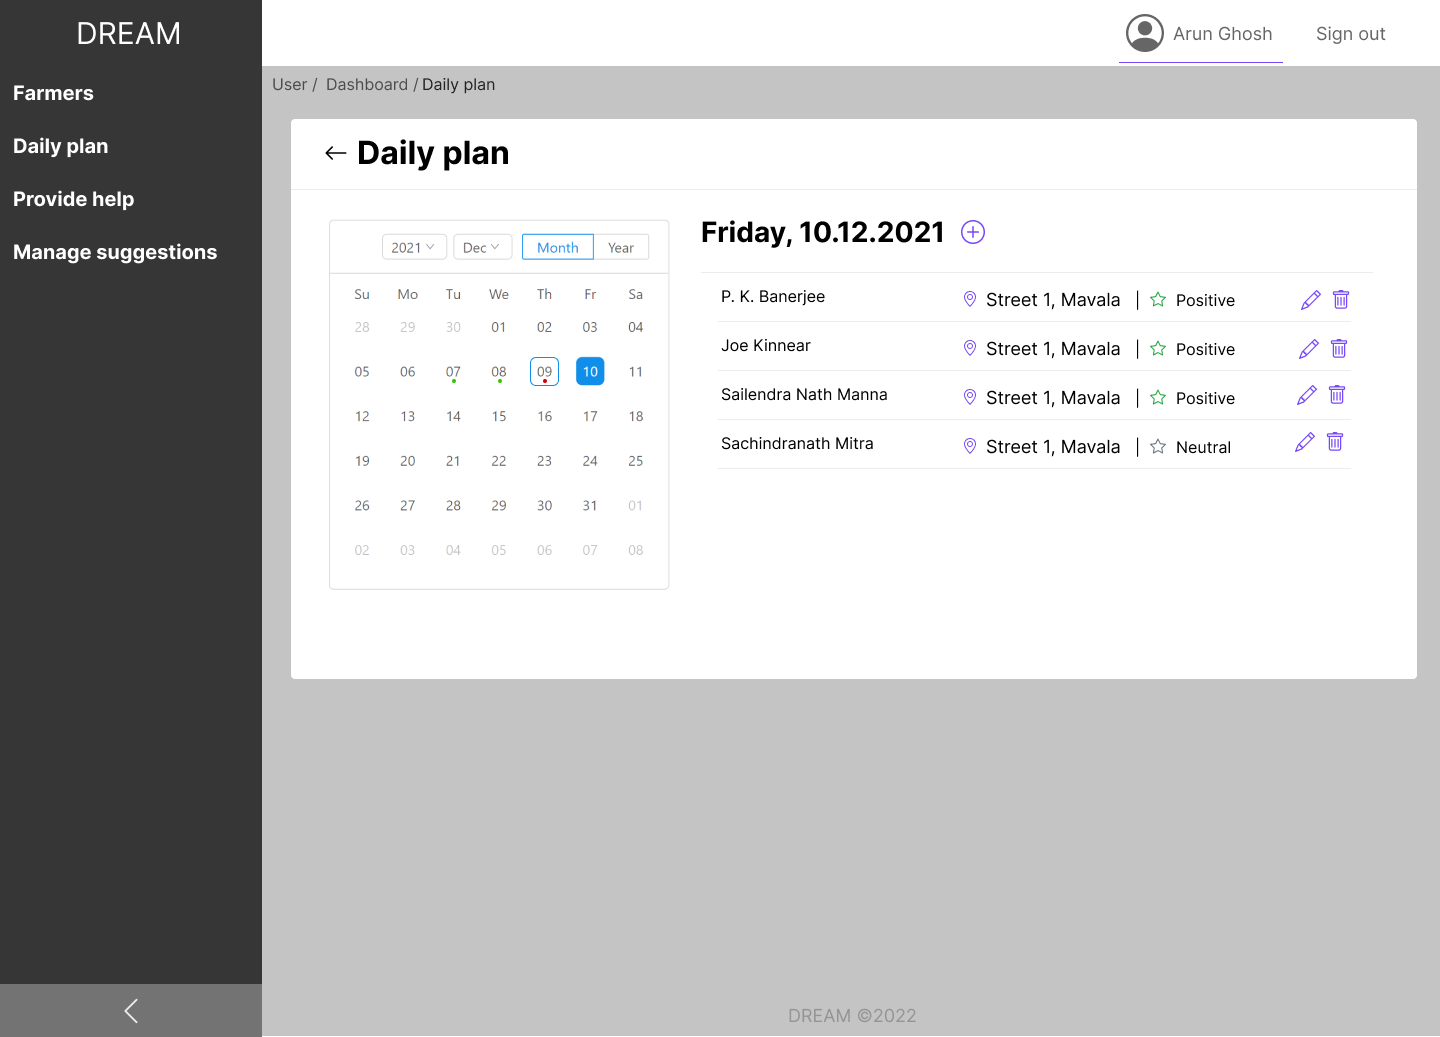
\includegraphics[width=0.75\textwidth]{mockups/Agronomist_Dashboard_Visit plan in future.png}
        \caption{\textbf{M21.} Calendar of daily plans – view of future day.}
    \end{figure}
    
    After clicking on the \textit{Submit execution state} button on the daily plan of today/past day, a modal dialog appears, allowing the agronomist to select, which farm he has visited and provide comments for farms he hasn't visited.
    \begin{figure}[H]
        \centering
        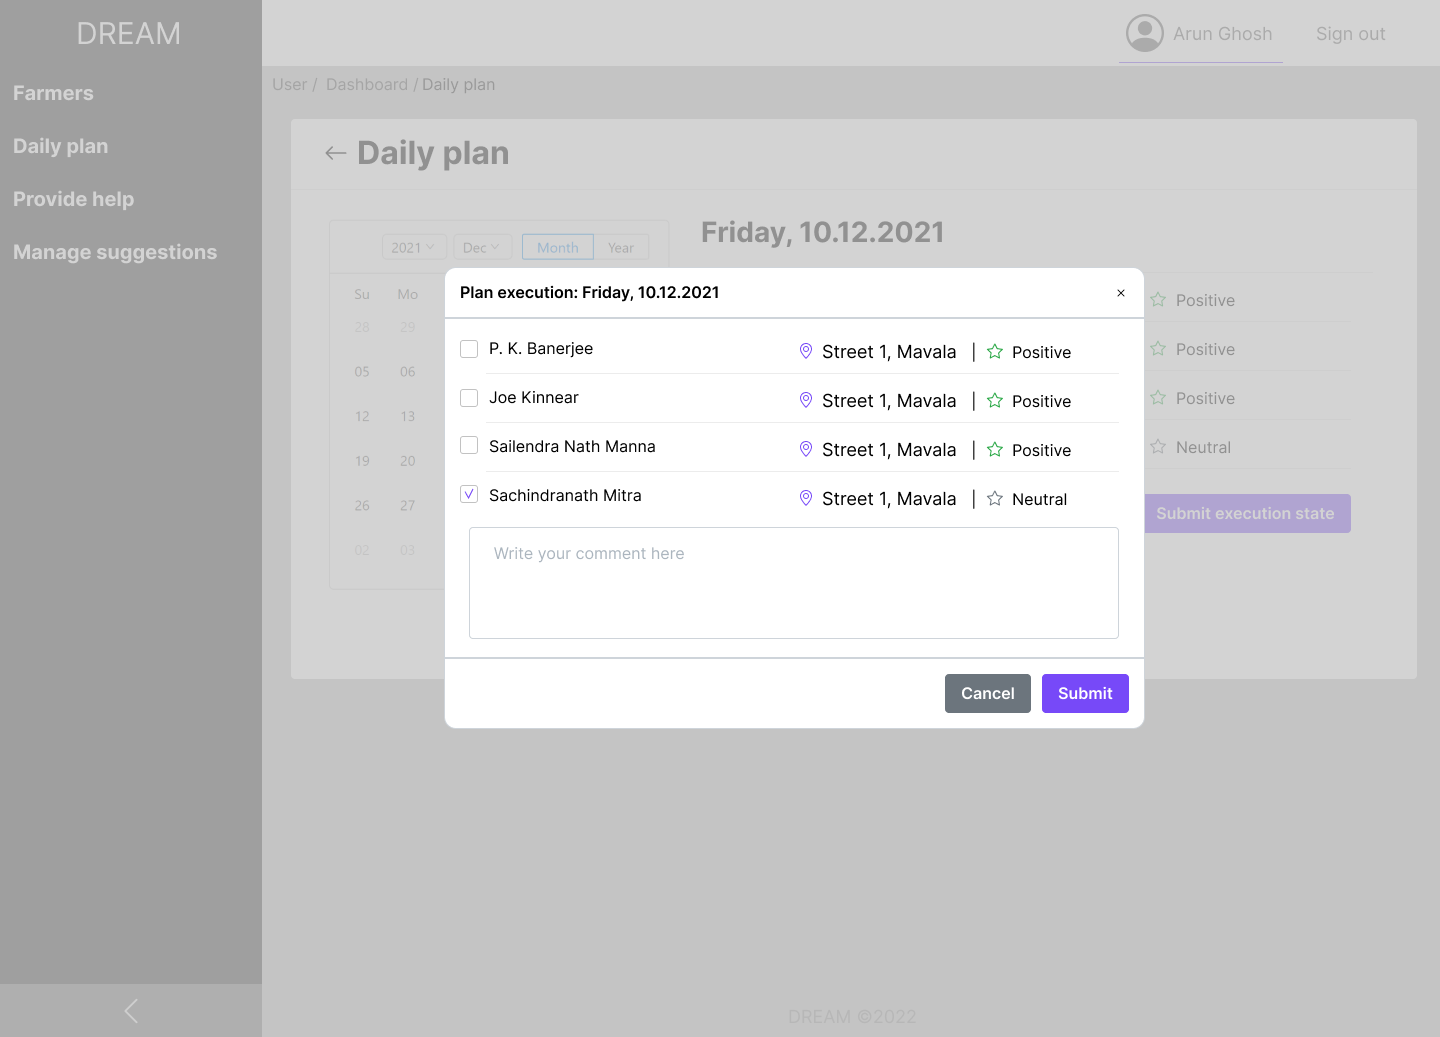
\includegraphics[width=0.75\textwidth]{mockups/Agronomist_Dashboard_Visit plan_Submit.png}
        \caption{\textbf{M22.} Submitting executions state of a daily plan.}
    \end{figure}
    
    The agronomist can view all received help request, by clicking on the \textit{Provide help} button in the left navigation bar. This view works exactly the same as the view available for farmers with positive note, presented in figure \ref{fig:farmer-provide-help}.
    \begin{figure}[H]
        \centering
        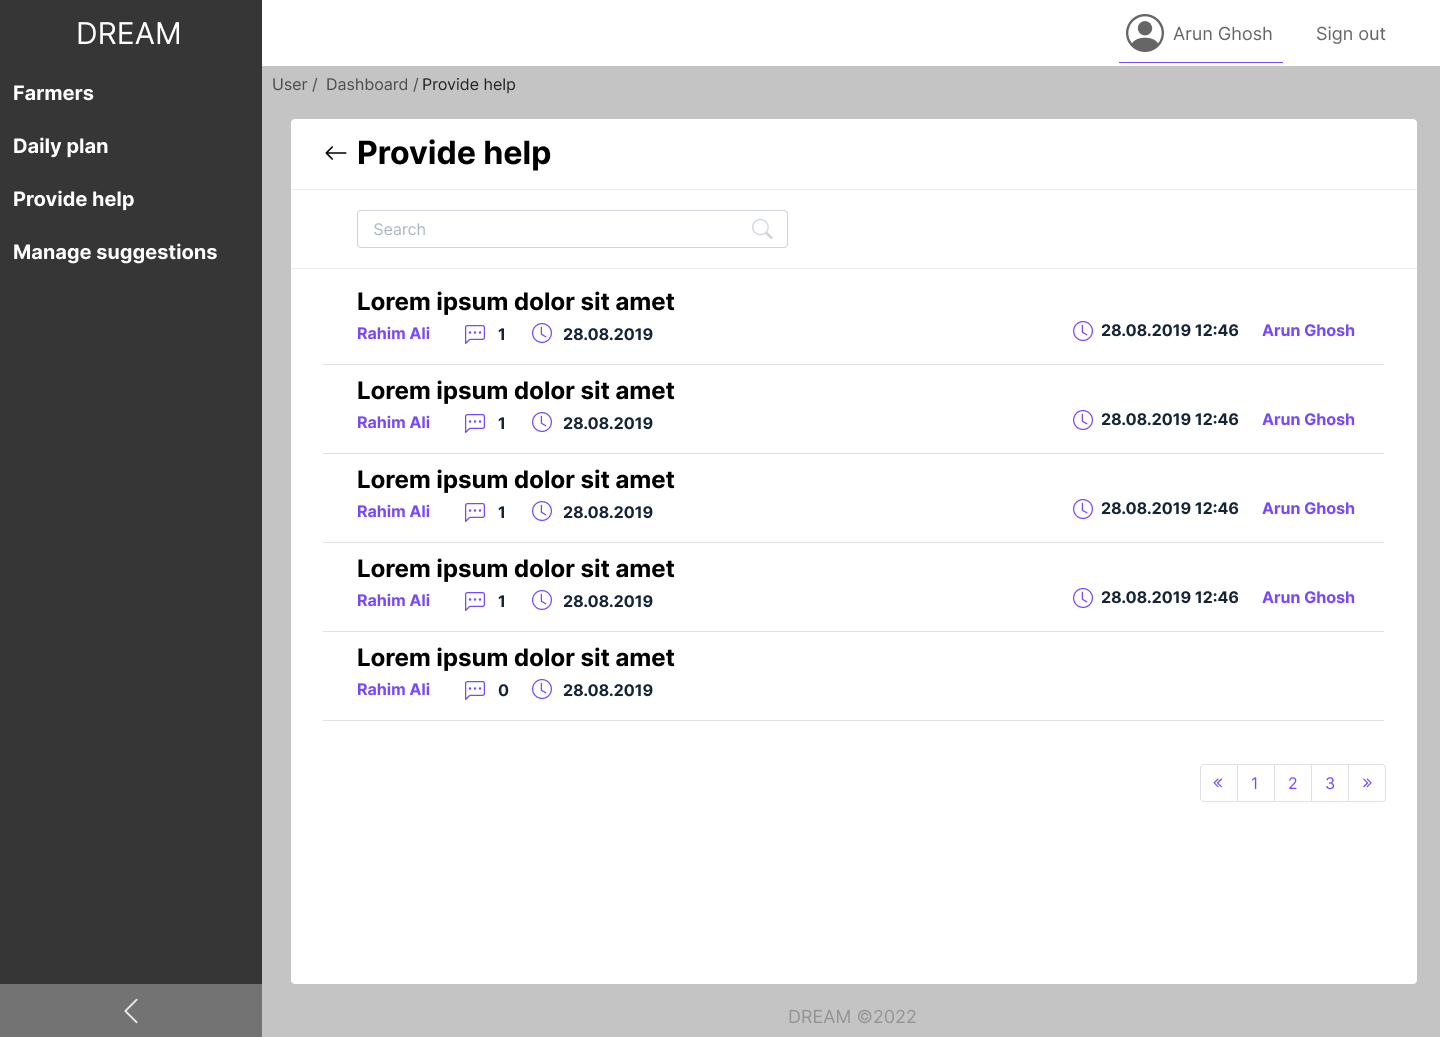
\includegraphics[width=0.75\textwidth]{mockups/Agronomist_Dashboard_Provide help.png}
        \caption{\textbf{M23.} Help requests received by agronomist.}
    \end{figure}
    
    The agronomist can manage suggestions available to farmers, by clicking on the \textit{Manage suggestions} button in the left navigation bar. Suggestions are presented in a table, containing mandals, corresponding production type as well as the suggestion itself. They can be edited, deleted, and added, using buttons next to entries or \textit{Add new} button in the lower part of the content card. During creation of the suggestion, the user can also choose types of weather, to which the suggestion corresponds.
    \begin{figure}[H]
        \centering
        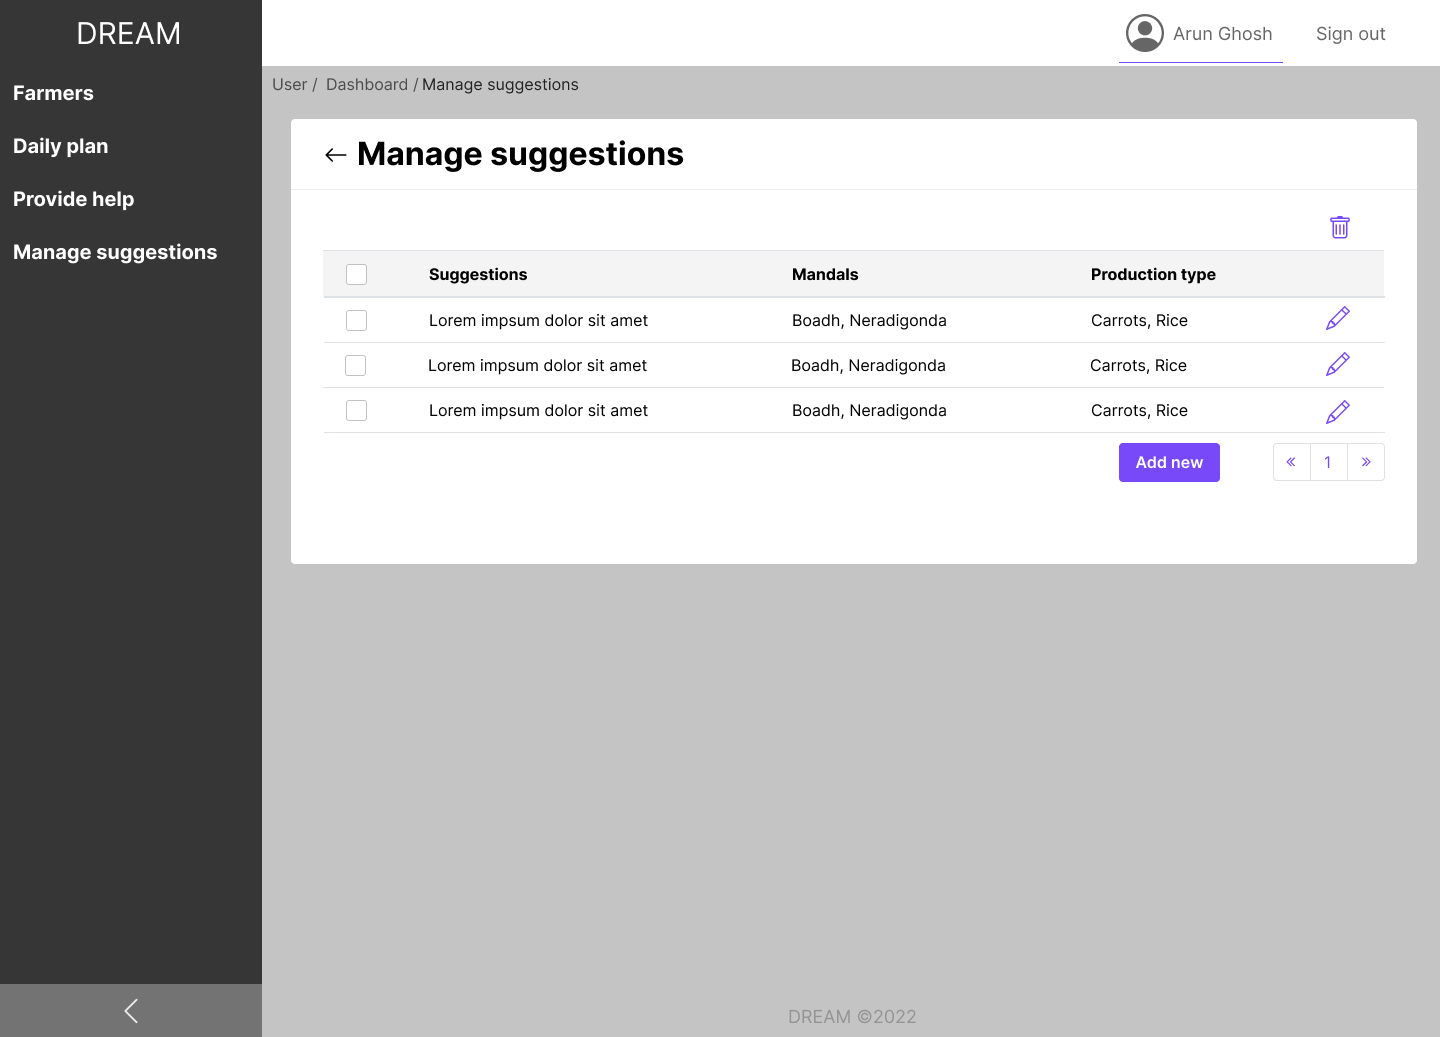
\includegraphics[width=0.75\textwidth]{mockups/Agronomist_Dashboard_Manage suggestions.png}
        \caption{\textbf{M24.} Managing suggestions.}
    \end{figure}
    
    \subsubsection{Policy maker}
    
    The policy maker can view his account summary, by clicking on the button in the top navigation bar, containing his name and surname. In the user view, he can view his account details and delete his account.
    \begin{figure}[H]
        \centering
        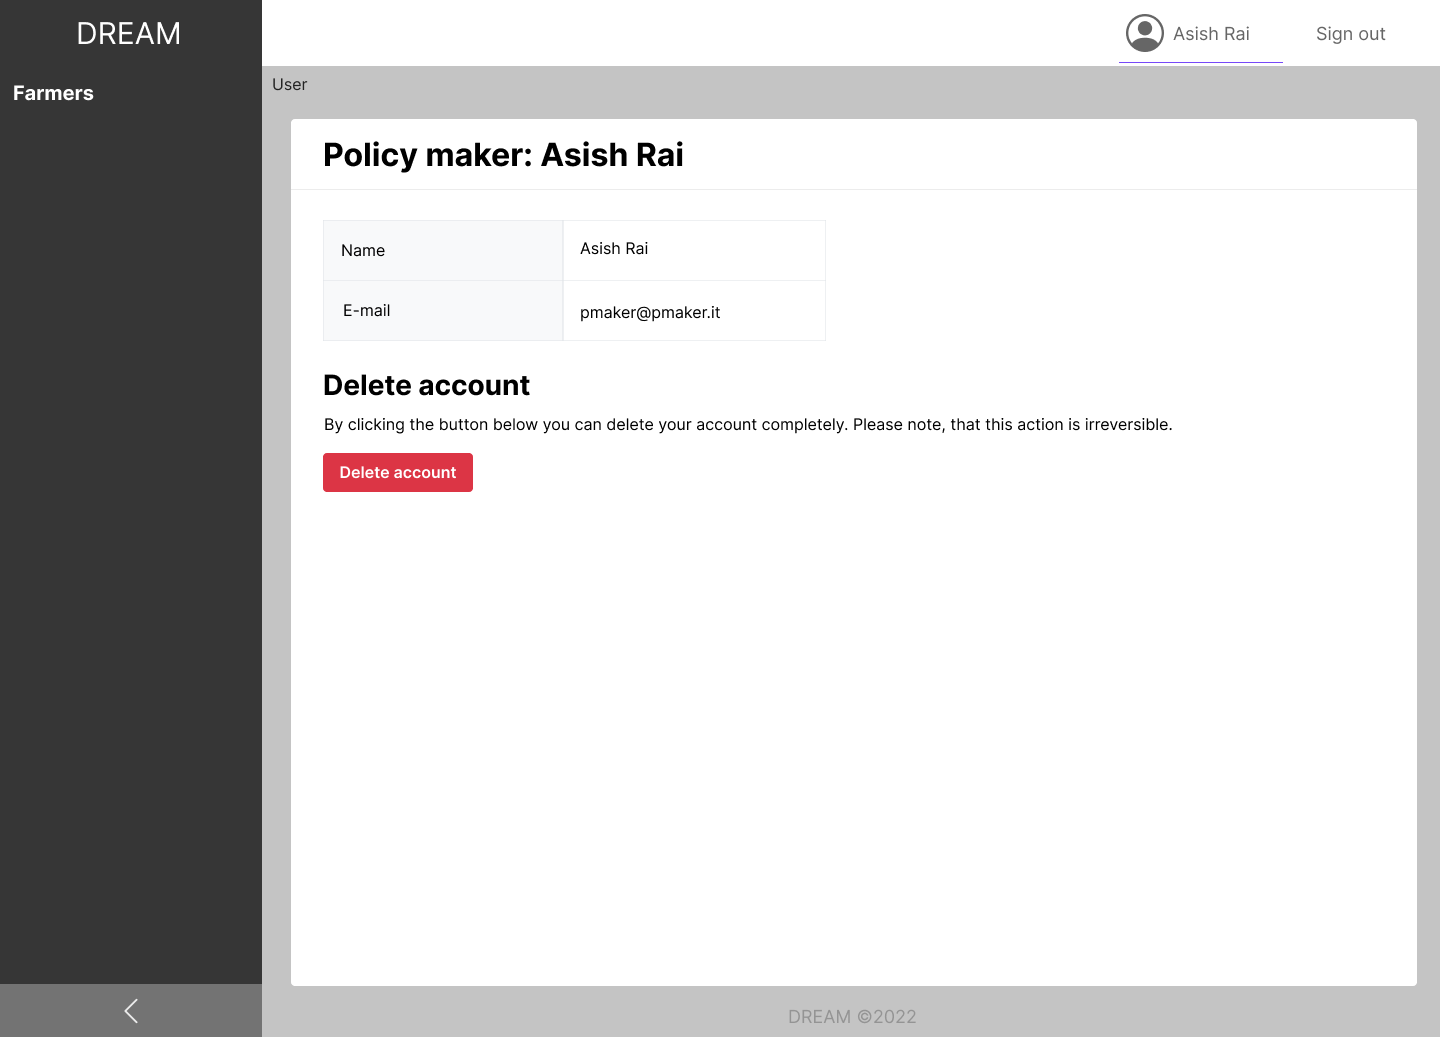
\includegraphics[width=0.75\textwidth]{mockups/Policy maker_User.png}
        \caption{\textbf{M25.} Policy maker's user view.}
    \end{figure}
    
    Directly after logging in, the policy maker is redirected to the dashboard view, which contains a summary of the well and bad prospering farmers in Telangana.
    \begin{figure}[H]
        \centering
        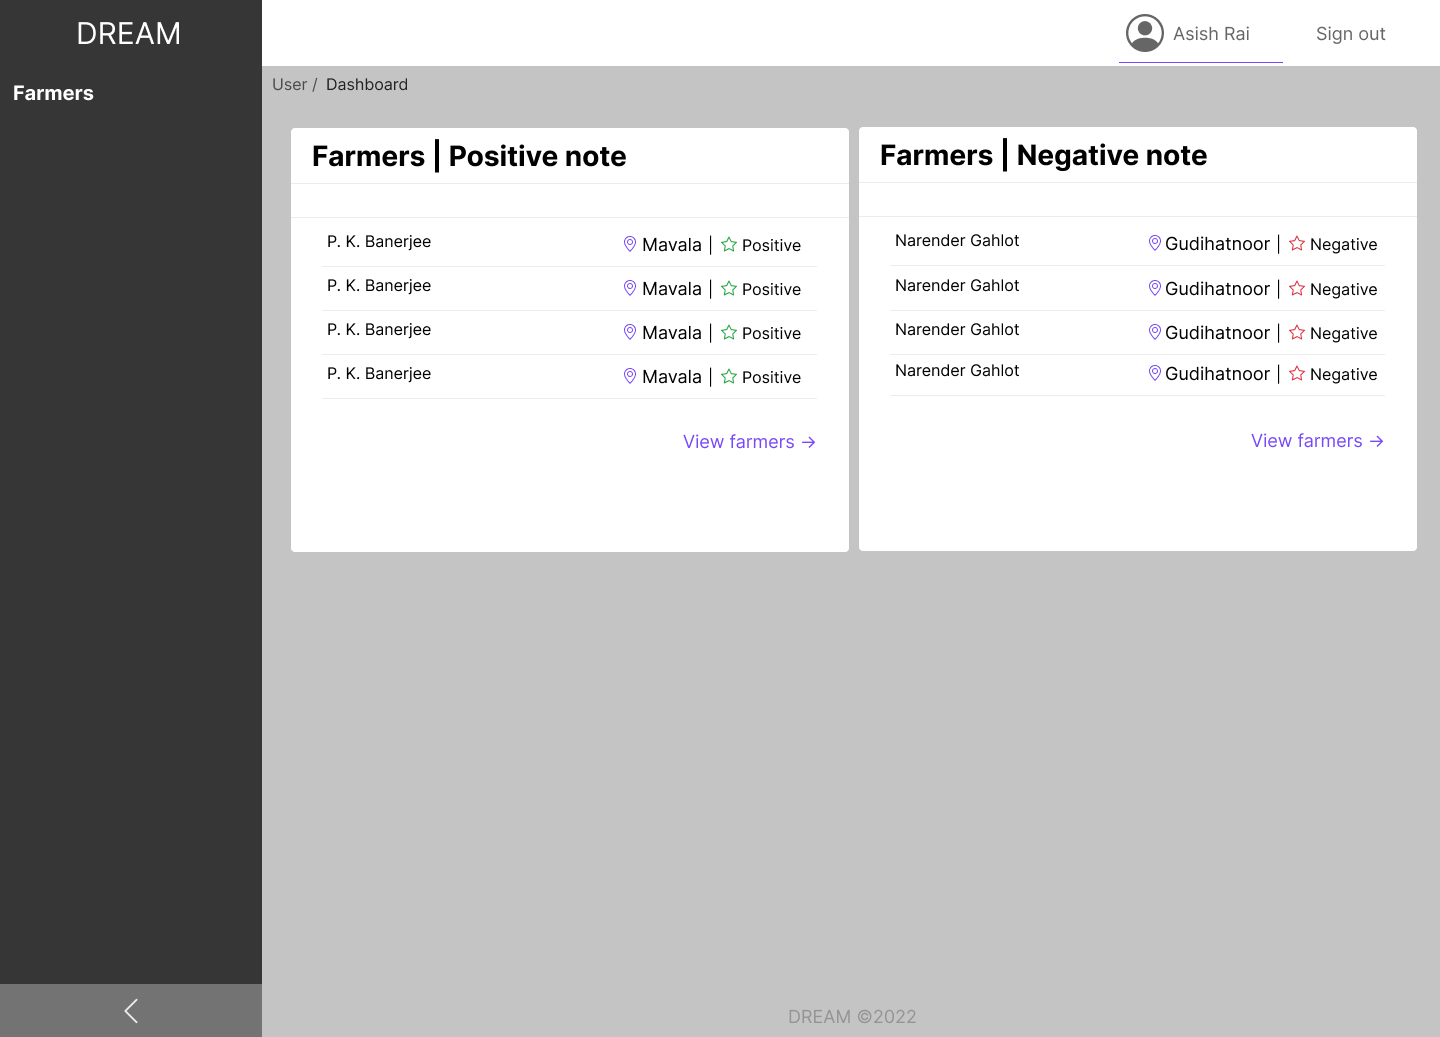
\includegraphics[width=0.75\textwidth]{mockups/Policy maker_Dashboard.png}
        \caption{\textbf{M26.} Policy maker's dashboard.}
    \end{figure}
    
    The policy maker can click on a farmer's entry in the farmer list, shown in figure \ref{fig:agronomist-farmer-list}. The following farmer's summary is identical to the one described in figure \ref{fig:farmer-summary}, with one difference – it allows the policy maker to assign a note, by clicking on the \textit{Change} button in the account details.
    \begin{figure}[H]
        \centering
        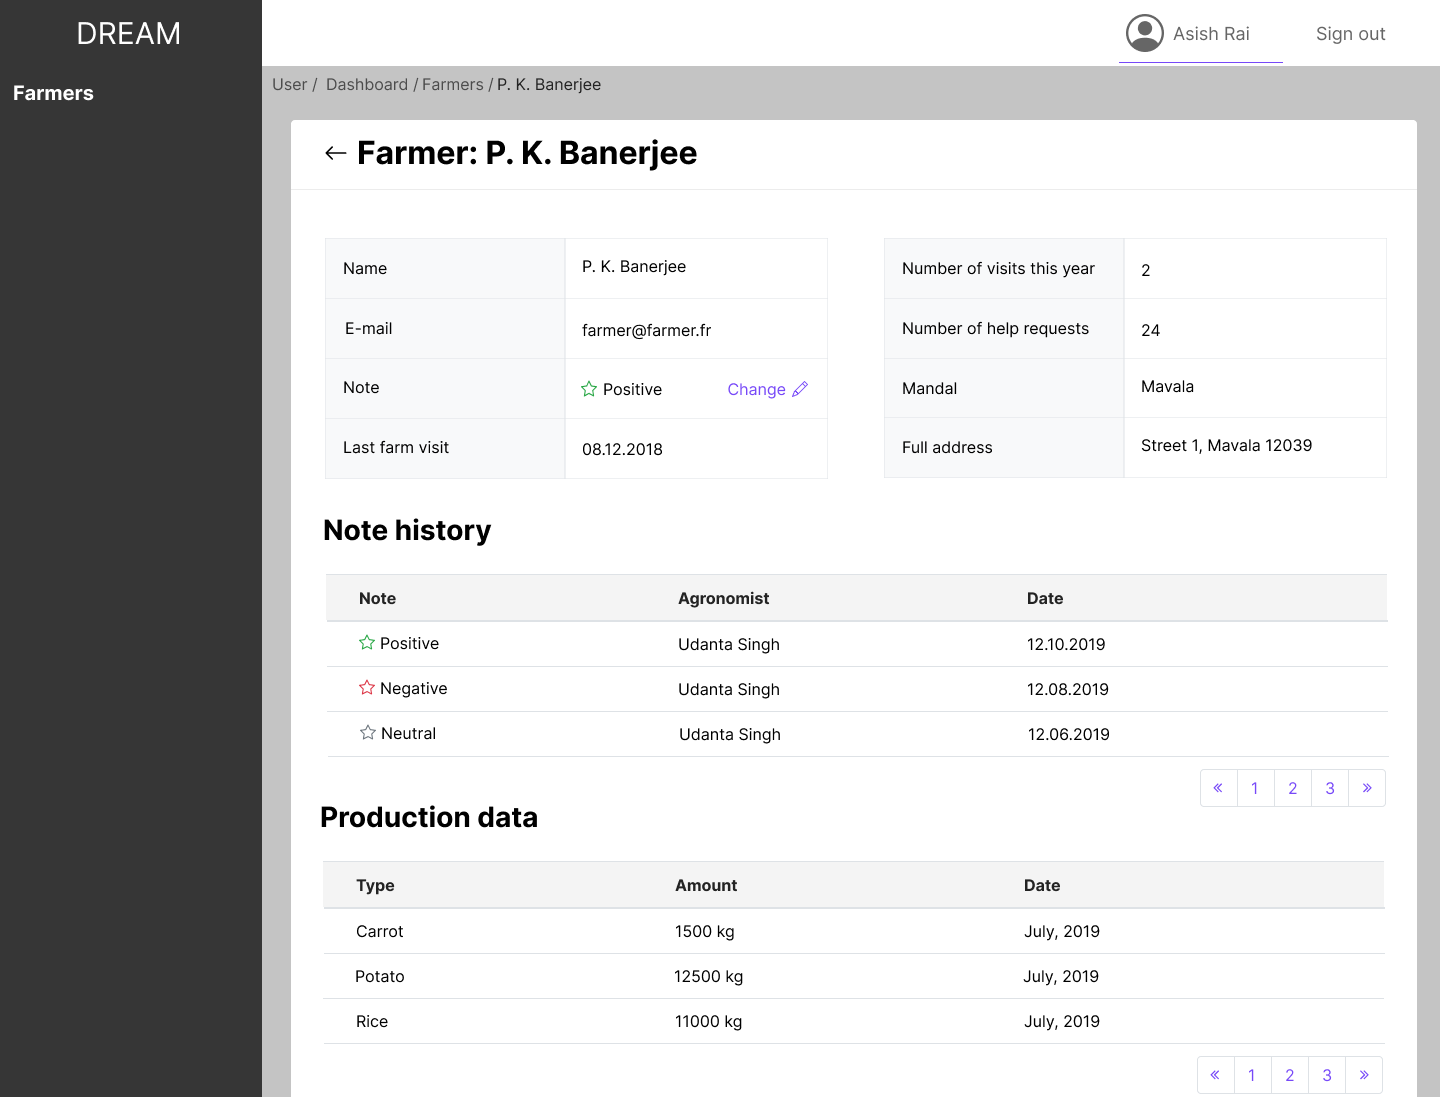
\includegraphics[width=0.75\textwidth]{mockups/Policy maker_Dashboard_Farmers_Farmer_part1.png}
        \caption{\textbf{M27.} Partial view of farmer's summary (applicable also to agronomist, without option to change note)}
    \end{figure}
    
    After clicking on the \textit{Change} button, a modal dialog appears. It allows the policy maker to choose a note and a problem type. In case of a negative note, a warning appears, informing the user of consequences of creating a negative note.
    \begin{figure}[H]
        \centering
        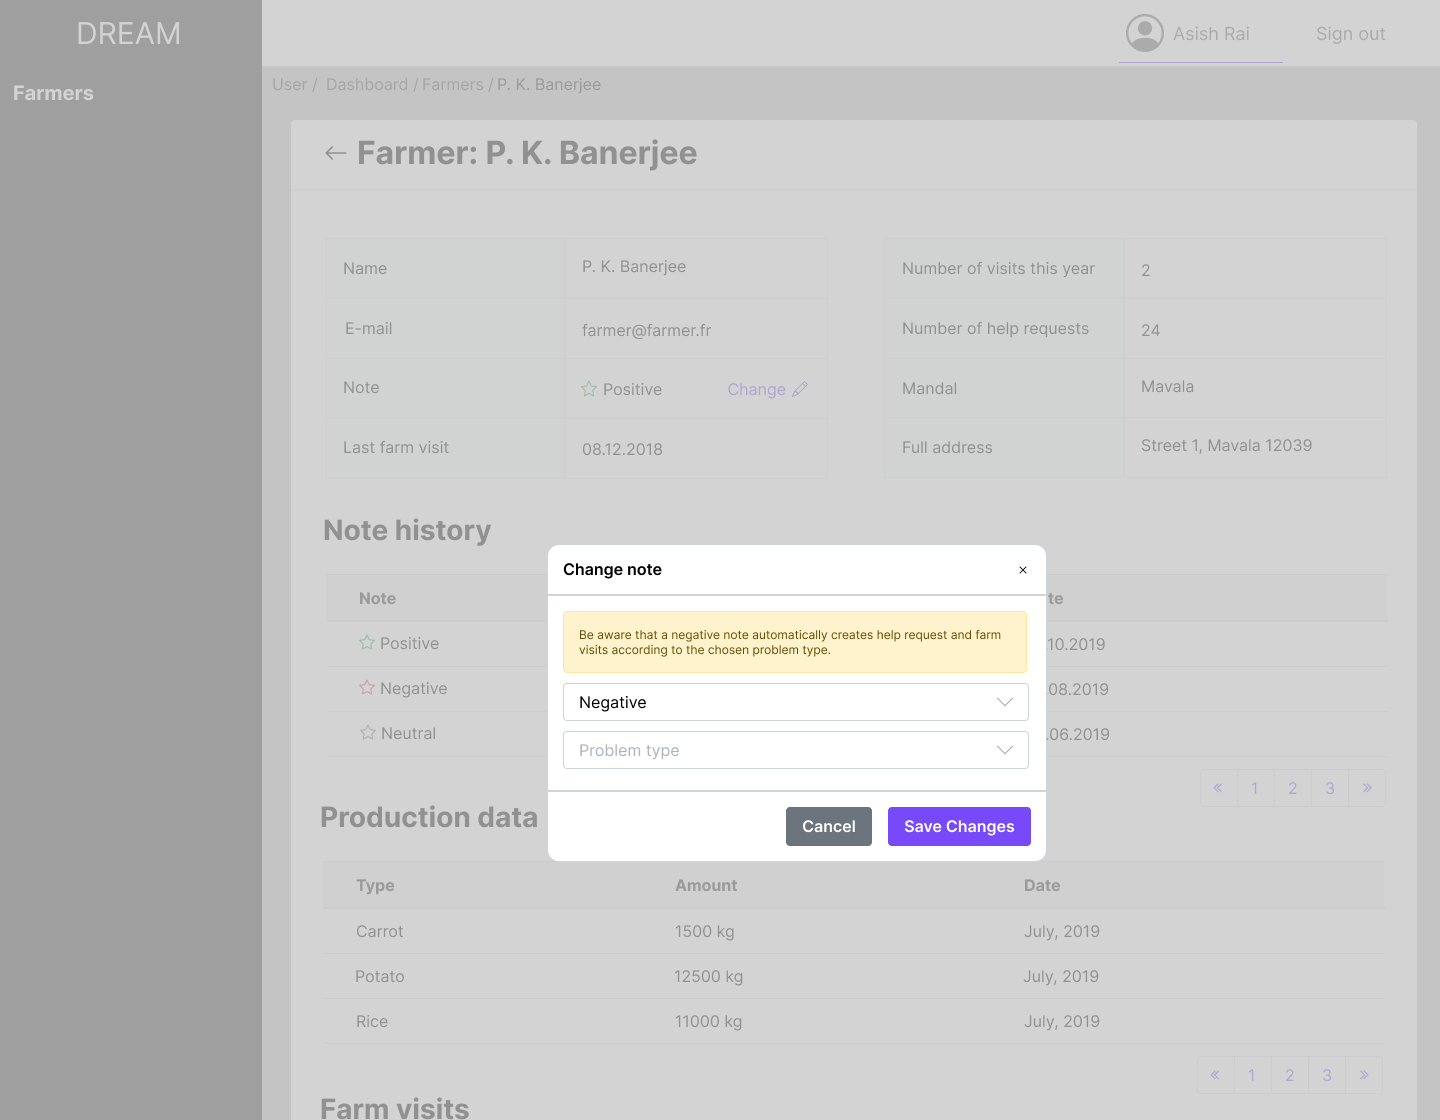
\includegraphics[width=0.75\textwidth]{mockups/Policy maker_Dashboard_Farmers_Farmer_Note_1.png}
        \caption{\textbf{M28.} Assigning note to farmer.}
    \end{figure}
